\section{Data and methods}
\subsection{General workflow}
\justify

A selection of web applications were designed and programmed for this thesis. In this chapter the process to create these applications is presented, from the design board to a functional web application to the end stage of data processing and visualisation. Four applications are presented in this chapter: a spatial web survey for data collection, and three separate web applications for the analysis and visualisation of the survey results.

Essential data for this research was provided by Statistics Finland, the research group Digital Geography Lab of University of Helsinki, the municipalities of Helsinki Capital Region, and Finnish Environment Institute. The research area of this thesis was based on PAAVO open data by postal code area (\cite{StatisticsFinland2019a}. Data such as the CORINE Land Cover 2018 artificial surface polygons and areas of urban structure were utilised to provide additional explanatory variables in the survey data (\textcolor{red}{cite corine}; \cite{Ristimaki2017}). For the visualisation of the survey results, various data by Statistics Finland was used (\cite{StatisticsFinland2012}).

Several programming languages were used to develop the survey web application and the subsequent data processing, analysis, and visualisation applications. The survey itself was created with HTML, JavaScript and PHP, with the essential help of Leaflet, a JavaScript mapping library (\cite{Agafonkin2019}). Data processing was a shared process between Python and R. Initial processing was done in Python and the analysis and visualisation in R. In Python, the library GeoPandas was in a central role, while interactive analysis and visualisation applications were created with the library Shiny (\cite{GeoPandasDevelopers2019}, \cite{Chang2019}). The thesis itself was written with LaTeX, a document preparation system, using the online LaTeX editor Overleaf (\textcolor{red}{cite}).

Initially, the research survey strove to collect parking event data on the precise temporal and spatial resolutions of an individual parking event and its exact coordinates, respectively. This first version of the survey created with Survey123 for ArcGIS was released to a small group of people before a planned larger roll-out, but it was quickly decided that a survey of a more general spatial and temporal resolution was needed to secure enough responses. After some consideration, one was programmed from the ground up using HTML and JavaScript. In this new survey, which was rolled out in May 2019, the respondent would send data about their parking activities in a specific postal code areas in a general sense, summing up their experiences in the most recent two years. The reduction in data resolution was substantial, but would still have more spatial fidelity than the existing parking time data in Helsinki Region Travel Time Matrix 2018 (\textcolor{red}{ttmcite}).

The survey was carried out in the four municipalities of Helsinki Capital Region. An invitation to participate in the survey was spread mostly in city district and neighborhood groups in Facebook. The response collection period continued until October 2019. The survey gathered, in total, 5222 responses from 4309 unique IP addresses.

After the conclusion of the data collection phase, the survey data was processed, analysed, and visualised using Python and R programming languages. The process started with anonymisation of the IP address data, and moved on to the processing proper. The objective of the data processing in Python was to bind the survey data with a selection of open spatial data in an effort to create additional explanatory variables for analysis.

The survey result analysis and visualisation was carried out in R. Utilising Shiny, a web application framework library for R, data analysis and visualisation applications were programmed for efficient and flexible data analysis for this thesis, but also to release the survey results to the public, maintaining the mission of openness and transparency of this thesis. \textcolor{red}{mieti josko avaisi shinyappien sisältöä tähän}

The general workflow of the thesis data processing can be viewed in figure~\ref{fig:gen_workflow}.

\begin{figure}[H]
    \centering
    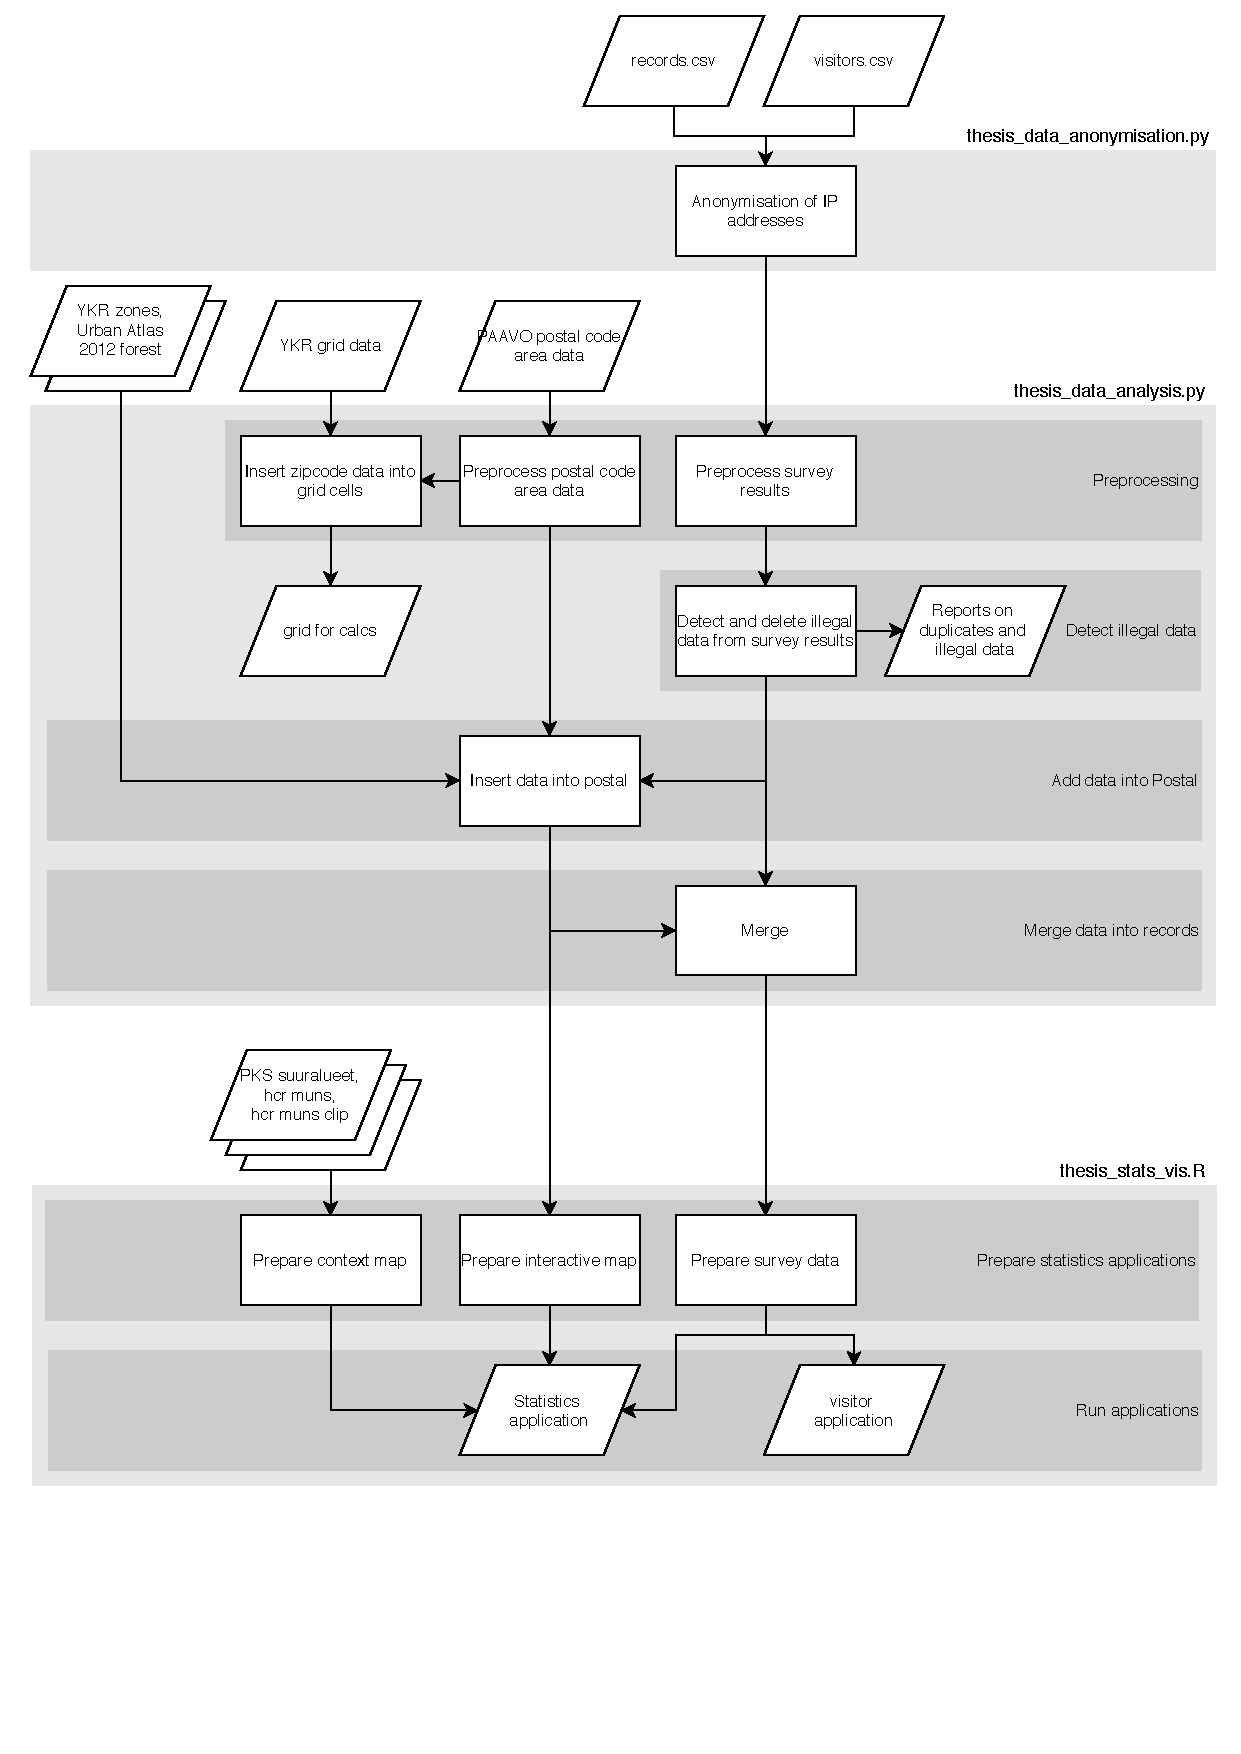
\includegraphics[trim=0.5cm 2.0cm 0.5cm 0.5cm,width=\columnwidth,scale=0.5]{thesis_workflow.pdf}
    \caption{The general workflow of the thesis survey data processing in Python and R.}
    \label{fig:gen_workflow}
\end{figure}
\pagebreak

\newpage
\subsection{Study area}
\justify
% https://www.hel.fi/hel2/Helsinginseutu/HS_tunnusluvut/liikennemaara_ja_autonomistus.pdf
% https://www.hsl.fi/sites/default/files/19_2016_auton_omistus_helsingin_seudulla.pdf
% https://www.hsl.fi/tutkimukset/muut-selvitykset
% http://pxnet2.stat.fi/PXWeb/pxweb/fi/StatFin/StatFin__lii__mkan/

\textcolor{red}{add content to this chapter} The study area of this thesis is the Helsinki Capital Region in Finland. It comprises of municipalities of Helsinki, Espoo, Vantaa and Kauniainen. The total population of the metropolitan area is 1.5 million \textcolor{red}{LÄHDE}. In practice, the whole area amalgamates as one complete functional area with boundaries of the municipalities indistinguishable at the street level. The Helsinki Capital Region faces increasing pressure to manage its traffic because \textcolor{red}{LÄHDE}. Of these four municipalities Helsinki is the hub, and considered to contain the only inner city features of the municipalities (\textcolor{red}{syke-urbanareas}). Espoo, Vantaa and Kauniainen mostly consists of suburban areas with occasional industrial areas and large shopping complexes placed throughout the area. The Helsinki Capital Region is served with a high-performance public transport system comprised of buses, train, subway, and tram in Helsinki. Recently, in 2017, the subway expanded from Helsinki to Espoo, triggering a new phase of quickly evolving cityscape in the surroundings of the new stations.

\begin{figure}[H]%
    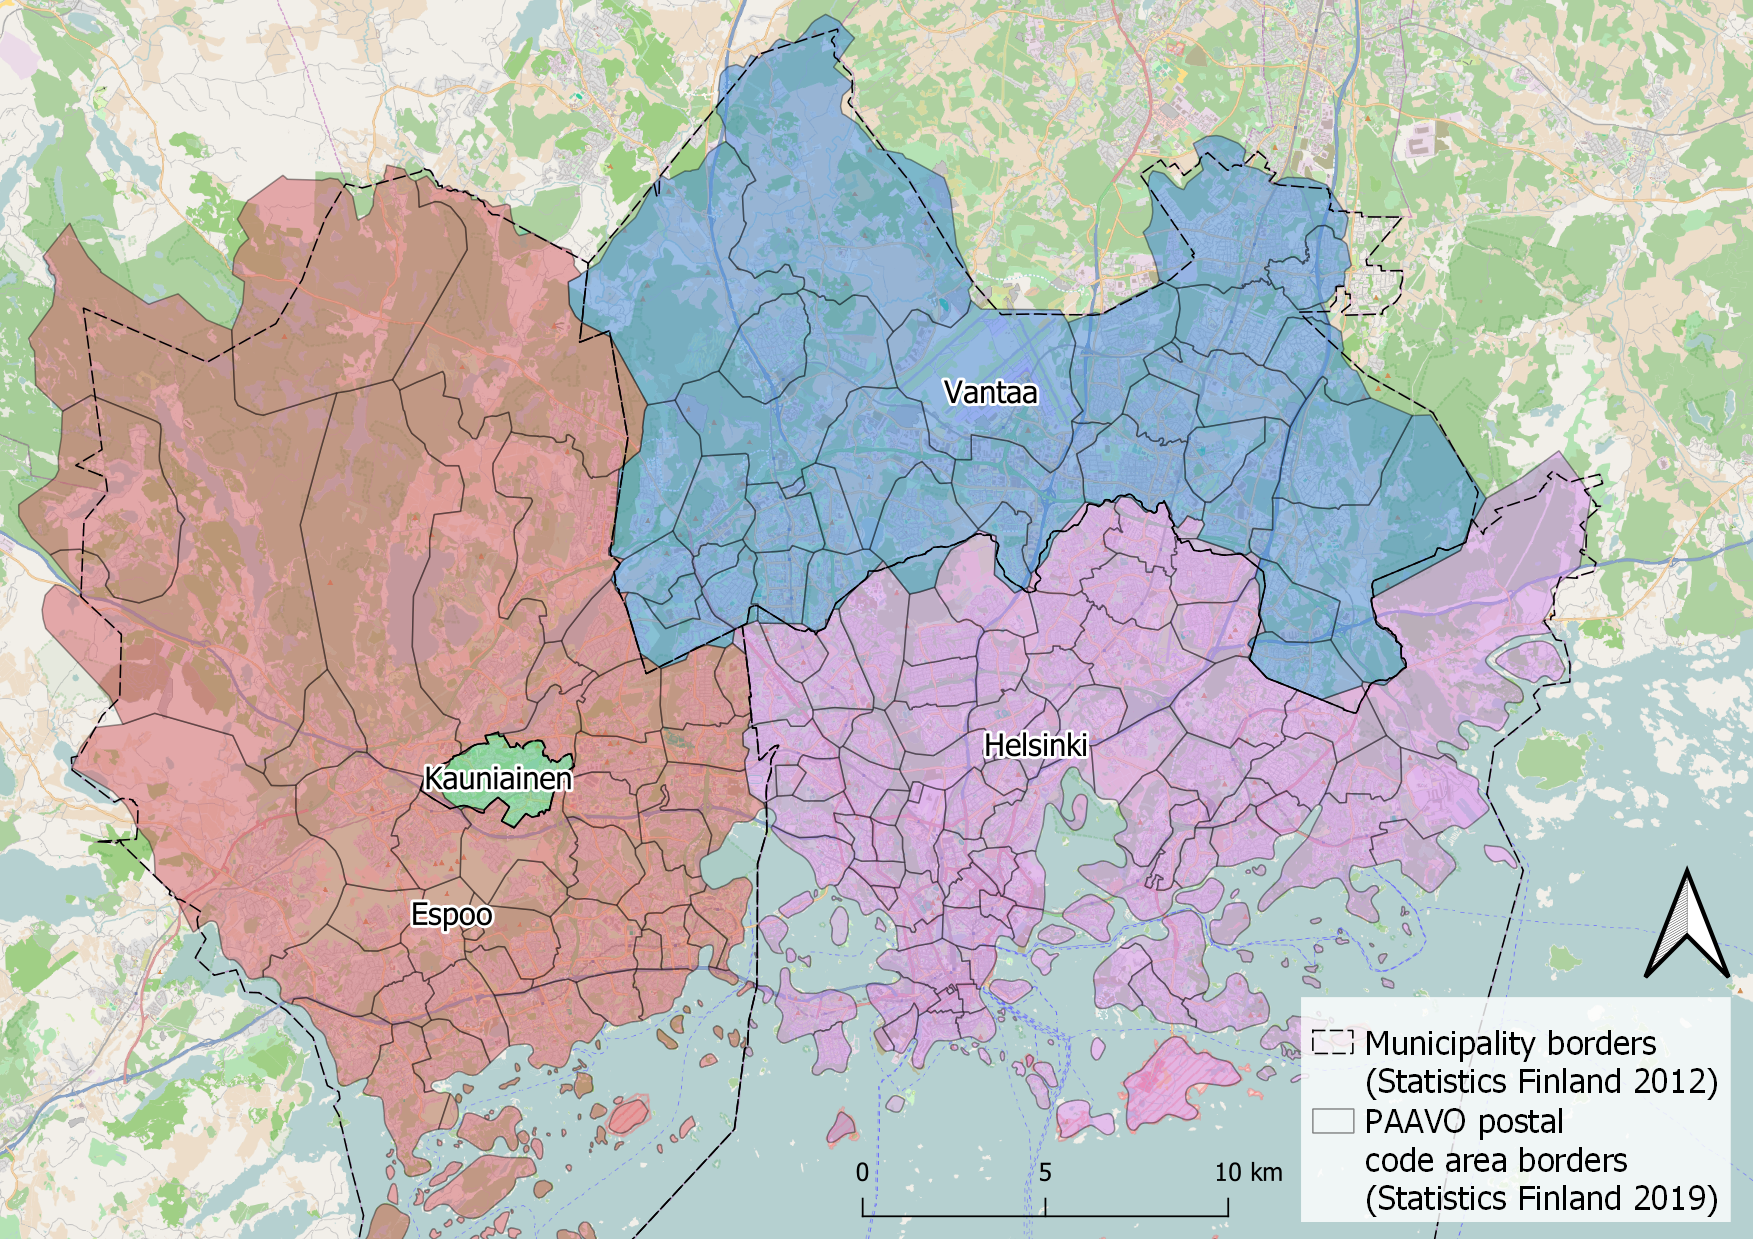
\includegraphics[width=\textwidth]{images/thesis_resarea.png}
    \caption[Research area map]{Map of the Helsinki Capital Region, the research area of this thesis. This research focuses on PAAVO postal code areas. The data has a municipality value for each postal code area (see the colouring of areas and map legend) but the areas do not completely align with the official municipality boundaries. \textcolor{red}{osmcite}}%
    \label{fig:thesis_resarea}%
\end{figure}

Despite the extensive service level of Helsinki Capital Region public transport, households especially in Espoo, Vantaa, and Kauniainen remain dependent on personal vehicles (\textcolor{red}{LÄHDE}). 

\newpage
\subsection{Data}
\justify

The foundation of this research is the dataset \textit{PAAVO -- open data by postal code area} (abbreviated \textit{postal} in this thesis) (figure~\ref{fig:paavo_resarea}). This data provides a large selection of data regarding the population of every postal code area in Finland. This includes detailed demographics and data about employment by field which follows the industrial classification TOL 2008 (\cite{Tilastokeskus2008}). However, this thesis only utilises the spatial definitions of the postal code areas, using these polygons to differentiate areas from each other in the web survey. This research makes use of the PAAVO 2018 dataset, released in January 2019.

In this thesis, the \textit{CORINE Land Cover 2018} (abbreviated \textit{CORINE}, figure~\ref{fig:datalayers}) vector format dataset is used to locate built area, or artificial surface, in the Helsinki Capital Region (\textcolor{red}{corinecite}). Provided by Finnish Environment Institute, CORINE contains polygonal data about land cover and land use for the entire nation in different hierarchy levels. In this thesis, the hierarchy level 1 value \textit{Artificial surfaces} is used. The minimum unit depicted in this dataset is 25 hectares in area or 100 meters in width. This slightly coarse data fits well with the spatially simplified nature of PAAVO postal code areas. CORINE dataset is an integration of automated satellite image interpretation and existing digital map data. \textcolor{red}{lisää taulukko siitä mitä level 1 artificial surfaces sisältää}

A main focus in this thesis was to compare the thesis survey results with \textit{Helsinki Region Travel Time Matrix 2018} (abbreviated \textit{TTM}), a dataset provided by Digital Geography Lab, a research group based in the University of Helsinki, the department of geosciences and geography (\cite{Tenkanen2018}). Their newest dataset provides travel times for public transport, private car, walking, and bicycling between all MetropAccess-YKR-grid cells (n=13231) \textcolor{red}{varmista että selitetty tätä ennen metropaccess ykr}. All travel times in this dataset were calculated using the door-to-door approach, which incorporates all parts of a journey from place A to place B into the travel time, including walking from one's home door to the car or bus stop and the time spent searching for parking. This thesis focuses on journeys made by private car.

\textit{MetropAccess-YKR-grid} (abbreviated \textit{grid}, figure~\ref{fig:datalayers}) is a spatial dataset consisting of cells with the dimensions of 250 by 250 meters (\cite{Toivonen2014a}). The dataset is used in the MetropAccess project of Digital Geography Lab and is based on the YKR data provided by Finnish Environment Institute and Statistics Finland (\cite{StatisticsFinland2020}). \textit{Grid} is a simple dataset and contains the spatial coordinates of cells and their identifiers, called the YKR ID. Using the YKR ID it is easy to connect \textit{TTM} data with the statistical data provided by Statistics Finland, allowing wide-ranging possibilities for further research.

All postal code areas in the survey results were classified with the \textit{zones of urban structures} (officially \textit{Yhdyskuntarakenteen vyöhykkeet}, abbreviated \textit{YKR zones}, figure~\ref{fig:datalayers}) (\cite{Ristimaki2017}). Utilising the same statistical grid of 250 x 250 meters as MetropAccess-YKR-grid, \textit{YKR zones} classifies grid cells to produce pedestrian, public transport, and automobile zones in and around Finland's urban regions using the theory of urban fabrics. According to this theory, these three zones developed during different times in the urban region's history (\cite{Newman2016}). In this thesis, every postal code area is assigned with a class defined in the \textit{YKR zones} based on which class has the largest presence. Adding this data into the survey results aimed to provide more possibilities to explain the hypothetical dissimilarity of survey results in different parts of the Helsinki Capital Region.

\textit{The regional division maps of Helsinki Capital Region} (officially \textit{Pääkaupunkiseudun aluejakokartat}, abbreviated \textit{subdivisions}, figure~\ref{fig:subdiv_placement}) was used in this thesis to analyse and visualise the survey results by subdivisions of Helsinki Capital Region (\cite{HelsinginEspoonVantaanjaKauniaistenmittausorganisaatiot2011}). Dividing the survey results into subdivisions would potentially give rise to local phenomena which would not be perceptible in the finest available level of spatial resolution, the postal code areas.

The dataset \textit{Regional population density 2012} (figure~\ref{fig:subdiv_placement}) was used in this thesis to visualise the boundaries of municipalities in Helsinki Capital Region (\cite{StatisticsFinland2012}). 

\begin{figure}[H]%
    \centering
    % use percentage of pagewidth with the syntax ".00\textwidth"
    \subfloat[CORINE Land Cover 2018 artificial surfaces in Kauniainen and eastern Espoo.]{{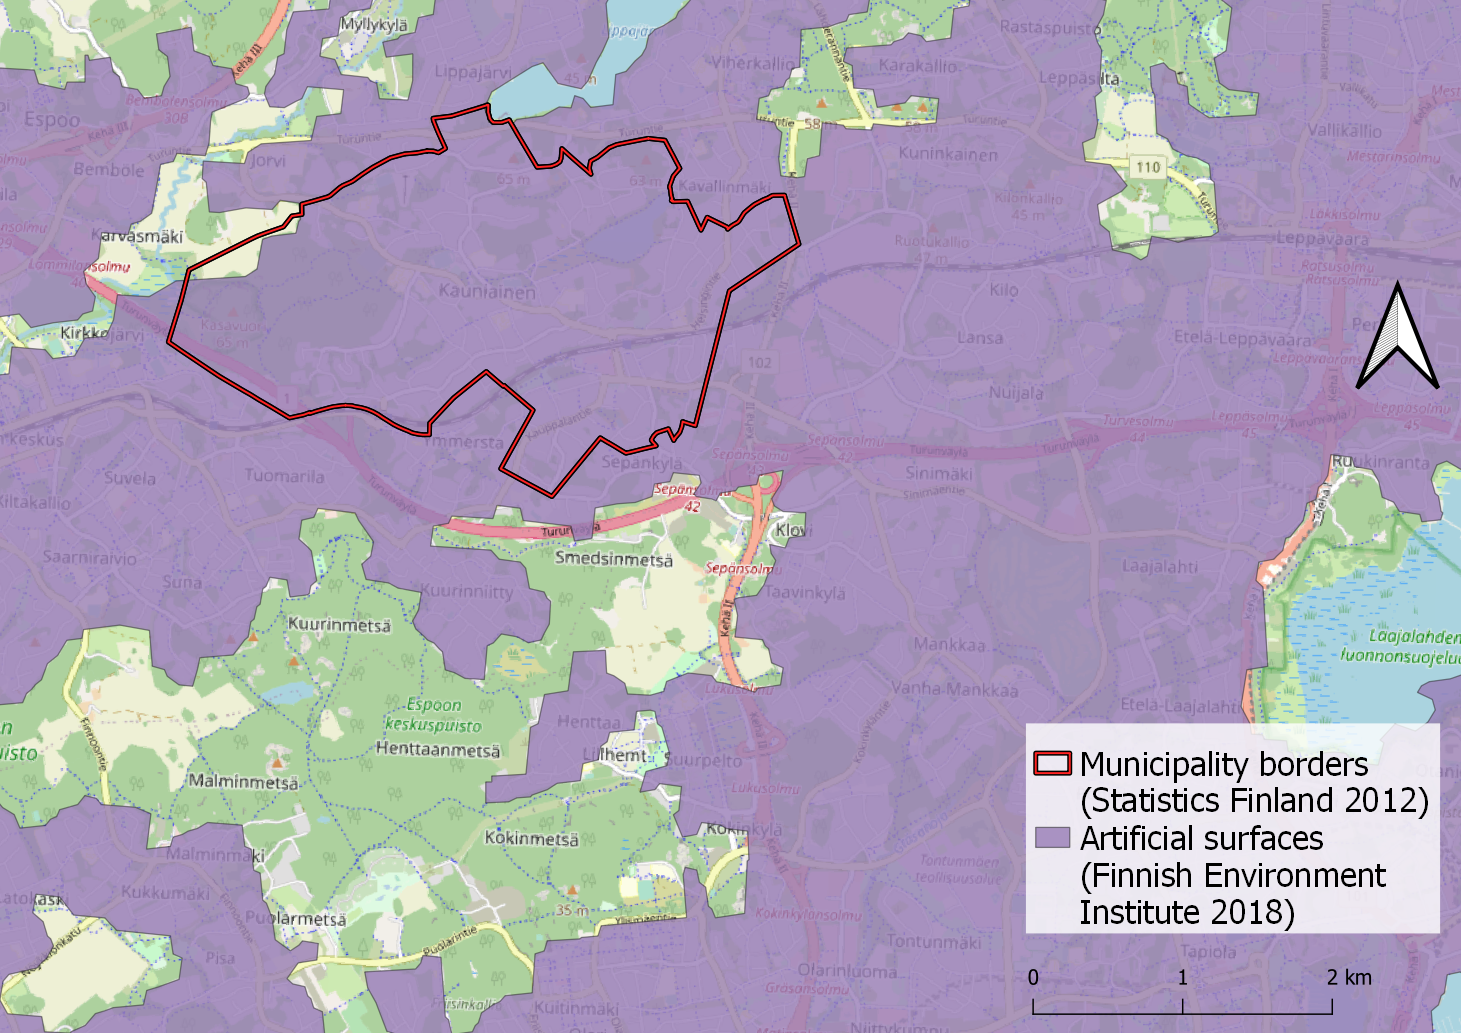
\includegraphics[width=.5\textwidth]{images/thesis_data_artificial.png} }}%
    \subfloat[Zones of urban structure in eastern Helsinki.]{{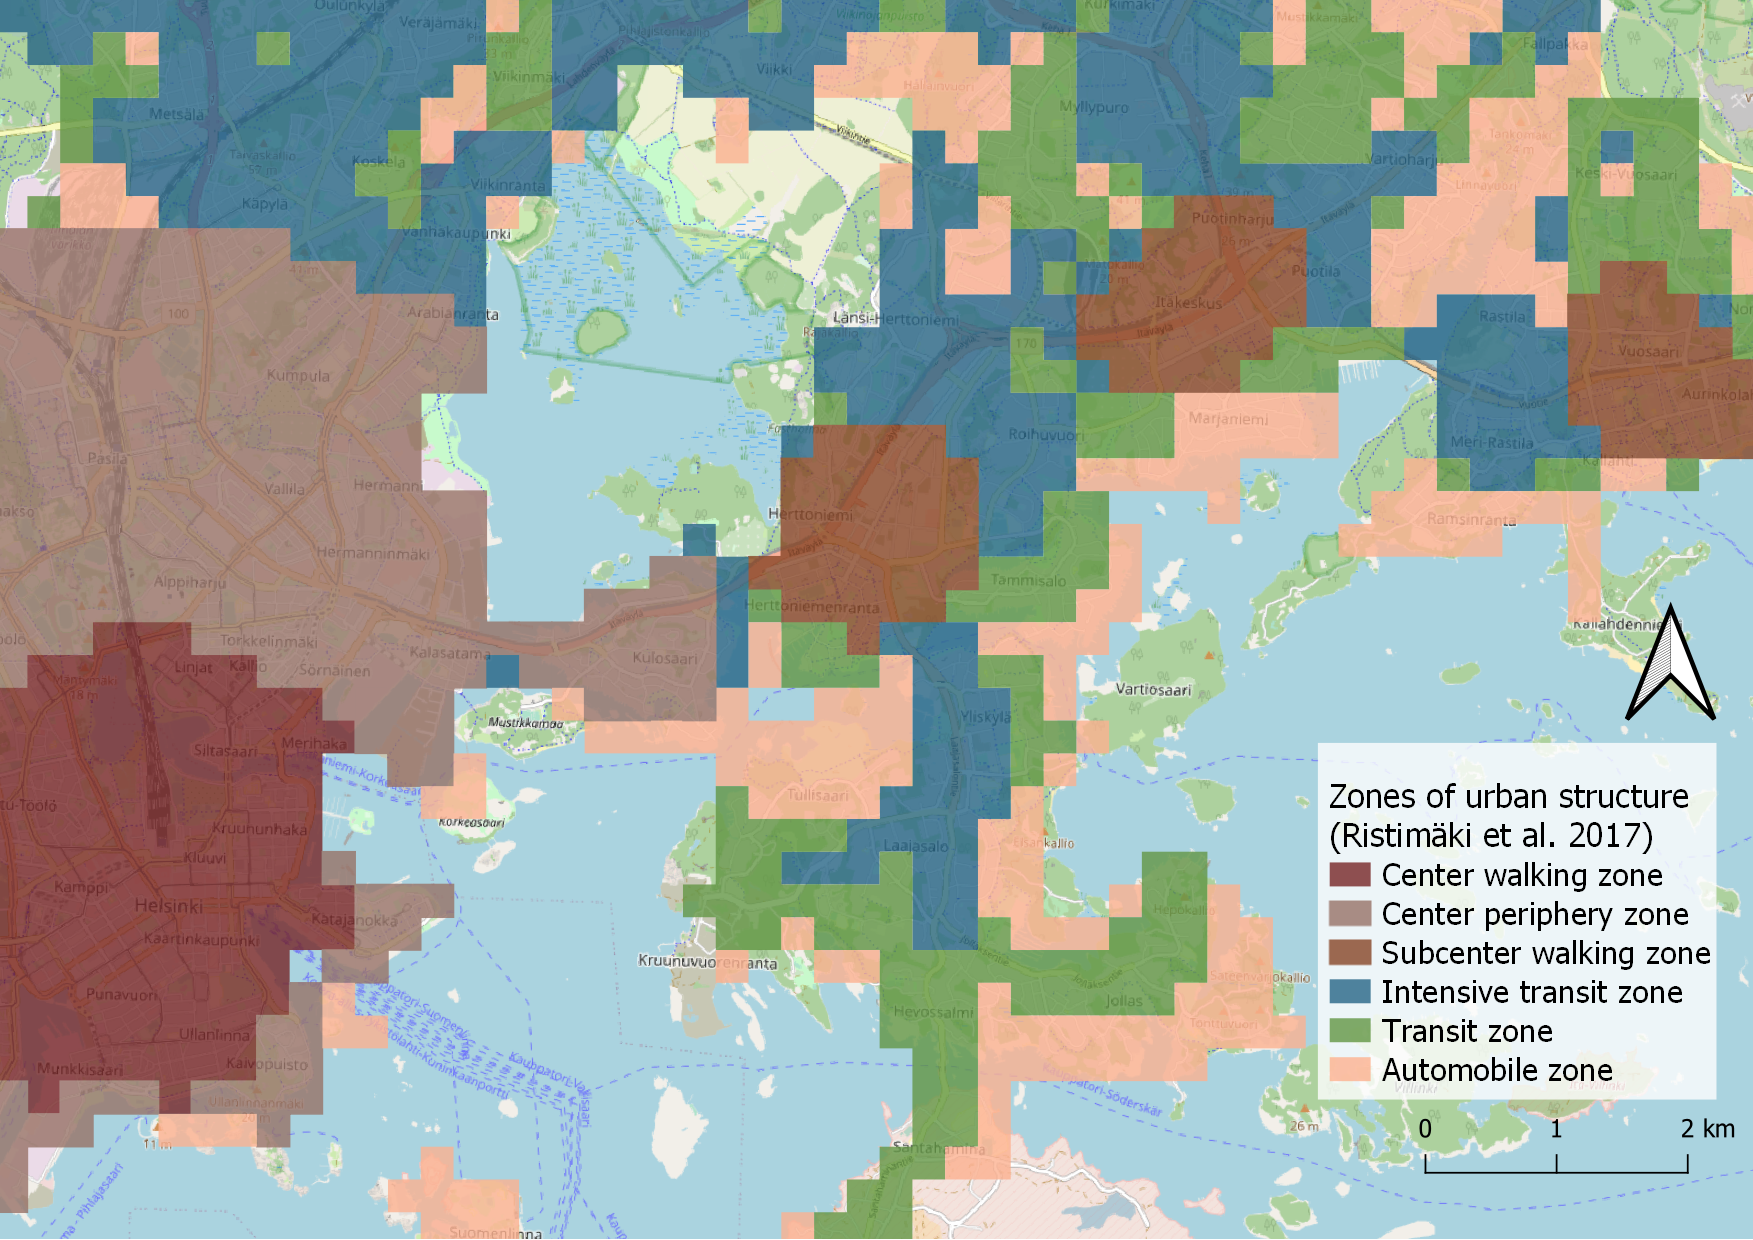
\includegraphics[width=.5\textwidth]{images/thesis_data_ykr_zones.png} }}%
    \quad
    \subfloat[MetropAccess-YKR-grid.]{{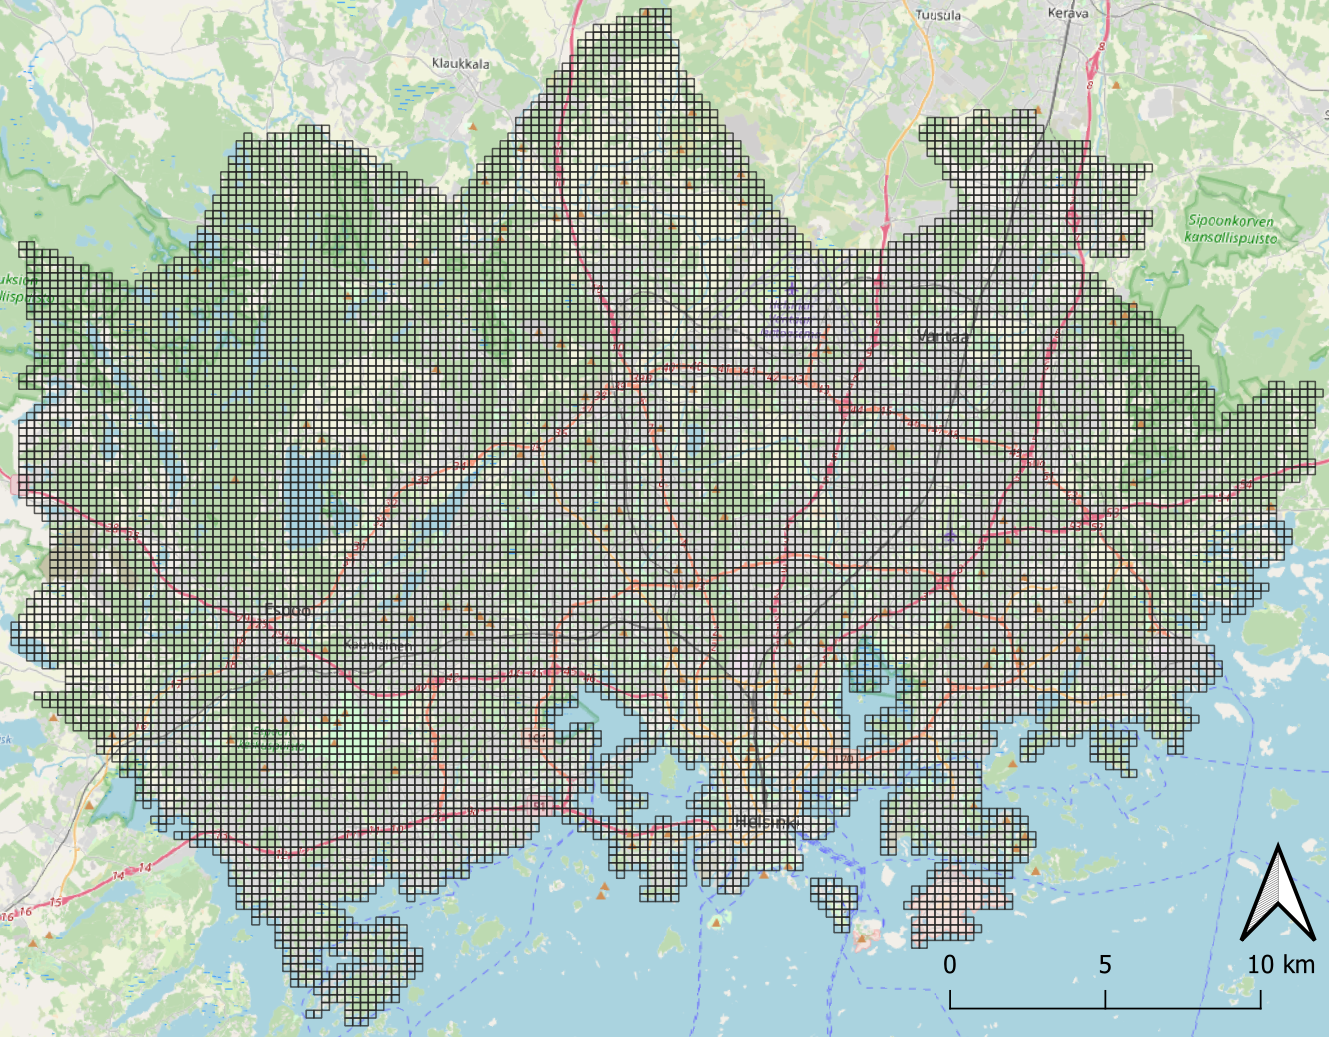
\includegraphics[width=\textwidth]{images/thesis_data_grid.png} }}%
    \caption[Spatial data]{Some of the spatial data used in the thesis. \textcolor{red}{osmcite}}%
    \label{fig:datalayers}%
\end{figure}

% hyphenrules: prevent hyphenation temporarily
\begin{hyphenrules}{nohyphenation}
    \begin{table}[H]
        \centering
        \caption[Thesis data]{Data utilised in the thesis.} 
        \label{tab:used_data}
        % use \scalebox{}{} to control table size. Note the additional curly brackets enveloping the entire tabular object
        \scalebox{0.8}
        % use \arraystretch to add whitespace between rows. \setlength\tabcolsep for columns
        {\def\arraystretch{1.5} 
        \setlength\tabcolsep{1.2ex}
        % One unit here is ">{\raggedright\arraybackslash}p{4cm}". \raggedright prevents justification of text and conveniently allows flush right or flush left, which is not possible with column command p{4cm} alone.
        \begin{tabular}{ @{} >{\raggedright\arraybackslash}p{4cm} >{\raggedright\arraybackslash}p{4cm} >{\raggedright\arraybackslash}p{4.5cm} >{\raggedright\arraybackslash}p{3.5cm} >{\raggedleft\arraybackslash}p{3.5cm} @{} }
            \toprule
            Data & Description & Purpose in thesis & Abbreviation in thesis & Citation \\
            \midrule
            CORINE land cover 2018 & Land use and land cover data in vector format & Artificial surface data & \textit{CORINE} & \textcolor{red}{cite} \\
            Helsinki Region Travel Time Matrix 2018 & Travel time and distance information for routes between all \textit{grid} cell centroids in the Capital Region of Helsinki & Use in travel time comparison calculations between \textit{TTM} and thesis survey results & \textit{TTM} & \cite{Tenkanen2018} \\
            MetropAccess-YKR-grid & Statistical grid of 250 x 250 meter cells for monitoring urban structure, Helsinki Capital Region area & Use in travel time comparison calculations between Travel Time Matrix 2018 and thesis survey results & \textit{grid} & \cite{Toivonen2014a}, \cite{StatisticsFinland2020} \\
            Paavo -- Open data by postal code area 2018 & Helsinki Capital Region postal code areas & Thesis research area and the basic unit of spatial resolution in the survey & \textit{postal} & \cite{StatisticsFinland2019a} \\
            Regional population density 2012 & Population density with municipality boundaries & Visualisation in R & \textit{hcr\_muns} & \cite{StatisticsFinland2012} \\
            Subdivisions of Helsinki Capital Region & The subdivisions of the municipalities of Helsinki Capital Region & Visualisation in R & \textit{subdivisions} & \cite{HelsinginEspoonVantaanjaKauniaistenmittausorganisaatiot2011} \\
            Zones of urban structure (Yhdyskuntarakenteen vyöhykkeet) 2017 & Delineation of urban areas based on the theory of urban fabrics & Data on spatial structure of urban areas & \textit{YKR zones} & \cite{Ristimaki2017} \\
            \bottomrule
        \end{tabular}}
    \end{table} 
\end{hyphenrules}

\newpage
\subsection{Used software}
\justify

A wide variety of software was used in the research for this thesis. The research strived for maximum openness and transparency and therefore much of the software employed in this work is free, open-source, or both. The research survey application utilised several essential web technologies such as JavaScript, HTML, CSS and PHP (table~\ref{tab:used_langs}). Using the web mapping library Leaflet, with the assistance of jQuery and other libraries, a modern and easy-to-use survey web application was created. Server-side, the programming language PHP was used to verify received data.

Data processing was carried out in Python 3.7.6 and R for Windows 3.6.3, with the initial processing done in Python and most of the analysis and visualisation in R (table~\ref{tab:used_langs}). Much of the work depended on additional software libraries available for the programming languages (table~\ref{tab:used_soft}). Python Anaconda version 2020.02 -- a distribution for Python for statistical computing -- provides the majority of the needed software libraries in the installation package, with the notable exception of GeoPandas, a library for geospatial pandas DataFrames in Python, and Shapely, a library for manipulation and analysis of planar geometric objects. In R, many libraries were used to achieve a comprehensive set of descriptive statistics. Libraries such as Shiny, ggplot2, and ggiraph formed the basis of the visualisation of the survey results.

% latex is not a programming language for the most part: https://www.quora.com/Is-LaTeX-a-programming-language
The thesis was written and typeset with LaTeX using the online LaTeX editor Overleaf. LaTeX is a document preparation system, used to create documents such as scientific articles. LaTeX adheres to the WYSIWYM (what you see is what you mean) system, as opposed to the "what you see is what you get" (WYSIWYG) system of text editors such as Microsoft Word, meaning that after establishing a set of parameters LaTeX will automatically compute the document formatting, while the user can concentrate on the document content. While LaTeX can be considered a programming language, it is more closely related to markup languages such as HTML (\textcolor{red}{cite}). In this LaTeX document, the LaTeX distribution TeX Live 2019 was used. Overleaf supports GitHub integration and as a result the complete thesis is available for viewing in the GitHub repository \textcolor{blue}{\url{https://github.com/sampoves/Masters-2020}} alongside with its entire development history. Additionally, the template of this thesis is provided at \textcolor{blue}{githublink, repo not started}.

In addition to the aforementioned technologies, the flowcharts in this thesis were created with the web application diagrams.net (\textcolor{red}{cite}). Most of the map visualisations of this thesis were made using the geographic information system application QGIS version 3.12.2.

% Consider! Removing \raggedright and hyphenrules will enable nice even table cells. Could be worth it to look into
\begin{hyphenrules}{nohyphenation}
    \begin{table}[H]
        \centering
        \caption[Thesis programming languages]{Programming languages, essential technologies, and \glspl{ide} utilised in the thesis, grouped by the function in this thesis.} 
        \label{tab:used_langs}
        \def\arraystretch{1.4}
        \setlength\tabcolsep{1.2ex}
        \begin{tabular}{ @{} >{\raggedright\arraybackslash}p{3cm} >{\raggedright\arraybackslash}p{4.5cm} >{\raggedright\arraybackslash}p{3.5cm} >{\raggedleft\arraybackslash}p{3.5cm} @{} }
            \toprule
            Programming language and \gls{ide} & Description & Purpose in thesis & Citation \\
            \midrule
            JavaScript, HTML, CSS (NetBeans 8.2.0) & Essential web technologies & Research survey programming, analysis and visualisation application programming & \cite{WHATWG2020}, \cite{W3C2020}, \cite{ECMA2019}, \cite{ApacheSoftwareFoundation2016} \\
            Python 3.7.6, Anaconda 2020.02 (Spyder 4.0.1) & Anaconda is a Python distribution for scientific computing & Survey data processing & \cite{Python3Reference}, \cite{AnacondaInc.2020}, \cite{SpyderProjectContributors2020} \\
            R for Windows 3.6.3 (RStudio 1.2.5033) & Programming language environment for statistical computing & Survey data analysis and visualisation & \cite{RCoreTeam2020}, \cite{RStudioTeam2015} \\
            LaTeX (Overleaf) & Document preparation system & Thesis formatting, structure, and writing & \textcolor{red}{latexcite, overleafcite} \\
            \bottomrule
        \end{tabular}
    \end{table} 
\end{hyphenrules}

\begin{hyphenrules}{nohyphenation}
    \begin{table}[H]
        \centering
        \caption[Essential software packages in thesis]{Essential software libraries used in the thesis. The complete list of libraries can be viewed in \textcolor{red}{appendix number something}.} 
        \label{tab:used_soft}
        \def\arraystretch{1.2}
        \setlength\tabcolsep{1.2ex}
        \begin{tabular}{ @{} >{\raggedright\arraybackslash}p{2.5cm} >{\raggedright\arraybackslash}p{3cm} >{\raggedright\arraybackslash}p{4cm} >{\raggedleft\arraybackslash}p{3cm} @{} }
            \toprule
            Programming language & Software package & Description & Citation \\
            \midrule
            % NB, manual positioning of the multirow label
            \multirow{3}{*}[-5ex]{JavaScript} & Leaflet 1.4.0 & Web mapping library for the research survey & \cite{Agafonkin2019} \\
            & jQuery 3.4.1 & Simplification of HTML DOM traversal and other features & \textcolor{red}{cite} \\
            & Font Awesome 5.13.0 & Font and icon collection & \textcolor{red}{cite} \\
            \greyrule
            \multirow{4}{*}[-6.5ex]{Python} & pandas 1.0.1 & Data analysis and manipulation & \cite{McKinney2011a} \\
            & GeoPandas 0.5.0 & Geographic data operations & \cite{GeoPandasDevelopers2019} \\
            & Shapely 1.6.4.post1 & Geometric objects, predicates, and operations & \cite{Gillies2019} \\
            & rtree 0.8.3 & Spatial indexing & \cite{Gillies2014} \\
            \greyrule
            \multirow{4}{*}[-7.0ex]{R} & Shiny 1.4.0.2 & Web application framework for R & \cite{Chang2019} \\
            & ggplot2 3.3.0 & Data visualisation & \cite{Wickham2016} \\
            & ggiraph 0.7.0 & Interactive ggplot2 graphics & \cite{Gohel2019} \\
            & dygraphs 1.1.1.6 & Interactive time series charting & \cite{Vanderkam2018} \\
            & fst 0.9.2 & High-performance writing and loading of data & \textcolor{red}{cite} \\
            \bottomrule
        \end{tabular}
    \end{table} 
\end{hyphenrules}

\newpage
\subsection{Methods}
\subsubsection{Considering survey development options}
\justify

To collect the areal parking data, the study required an interactive survey which respondents could use to submit their parking habits in a spatial fashion. To attract a largest possible number of submissions, the survey also needed to be of modern design, easy to use and its purpose easy to understand. The survey would have to be clear-cut, effortless to internalise and short in length as to prevent users getting frustrated and leaving before submitting answers. Design-wise, the spatial resolution of the survey was in question. The particular concern was that in the case of insufficient amount of answers, what kind of area delineation would be at the same time detailed enough but also streamlined enough to realistically reach results of good quality? This chapter strives to describe the process that would lead to the implemented web survey to accentuate the challenges this kind of research entail.

Once the consideration into options to produce the survey for this study had started, it quickly became apparent that there were few alternatives available and even fewer free, sufficiently customisable alternatives. Out of the proprietary options, Maptionnaire by the Finnish company Mapita was considered. They offer tailored map survey products with discounts for students. In return for the fee, a subscriber receives a time window in which to carry out their survey accompanied with tailored features and customer support -- the extent of features and support is determined by the price plan. The offered price was considered too steep for the thesis and Maptionnaire was passed on. 

Next Survey123 for ArcGIS was evaluated. An Esri operated service, Survey123 is used to create and analyse form based surveys (\cite{Esri}). It is included in the contract between University of Helsinki and Esri and thus was free to use for the study. One can quickly design a survey at the Survey123 website and share it immediately to respondents. Alternatively, the service is available as a desktop client, the Survey123 Connect, where Survey123 offers a wider range of possibilities for customisation with its adherence to the XLSForm standard. XLSForm is a standard to make authoring forms in Excel easier. With the customisability of XLSForm, users can design Survey123 surveys to the dot while employing the support for Excel style scripting for complex survey behaviour (figure~\ref{fig:survey123_xlsform}). Furthermore, Survey123 provides online tools for collaboration, analysis, and data viewing with many options for exporting the collected data.

\begin{figure}[H]%
    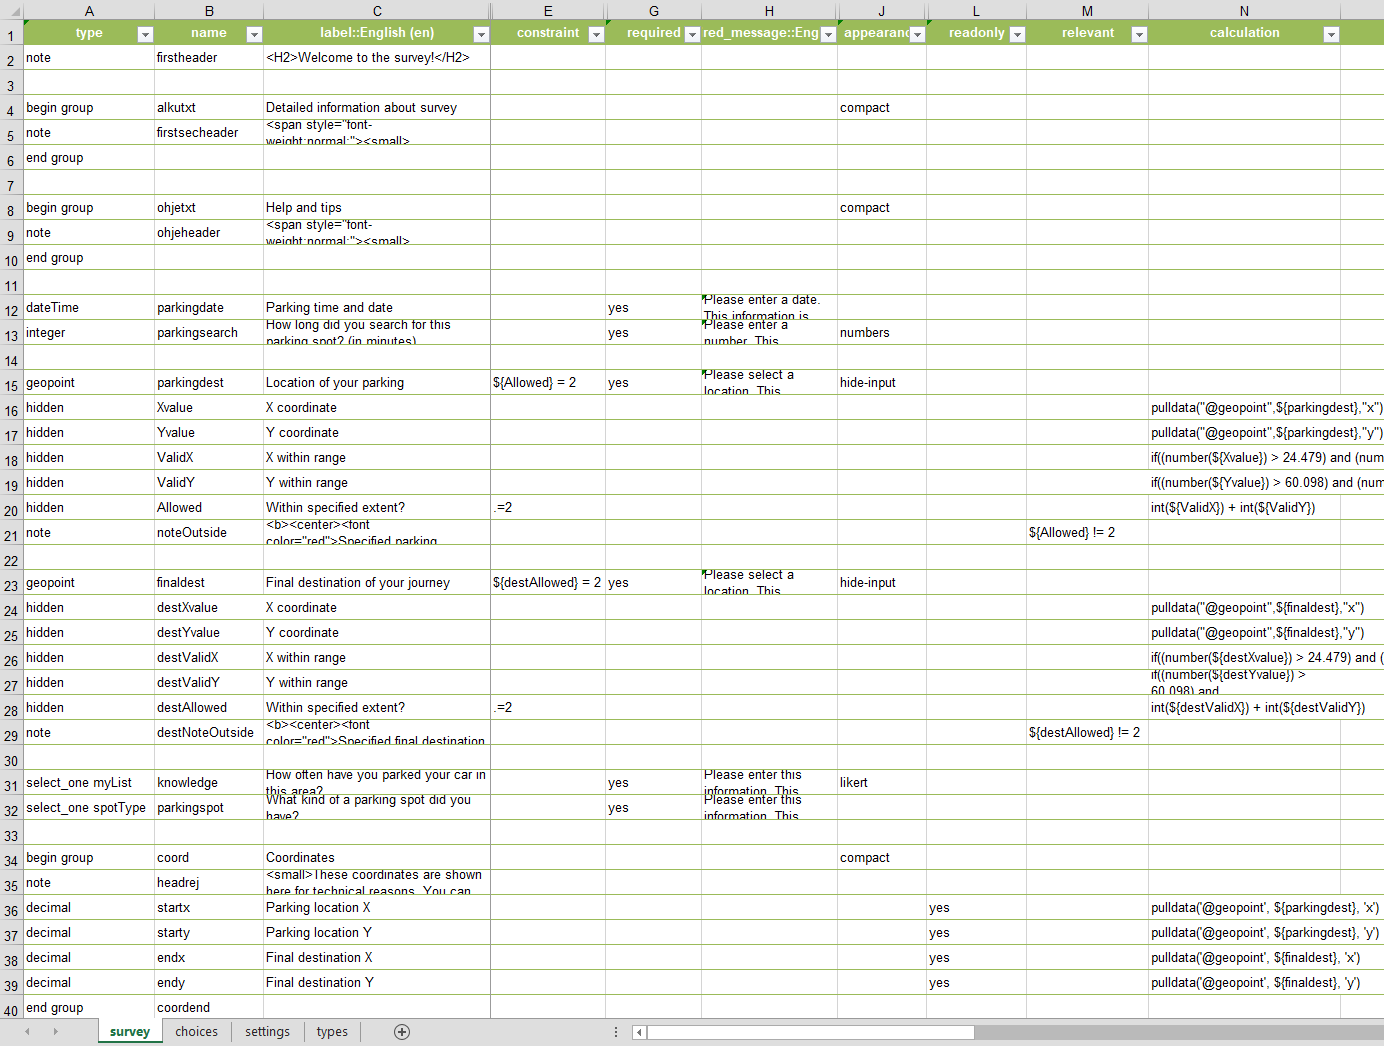
\includegraphics[width=\textwidth]{images/survey123_xlsform.png}
    \caption[Survey123 XLSForm view]{Survey123 XLSForm view in Microsoft Excel. Some parameter columns here are hidden to provide a view to the essential inner workings of the Survey123 form.}%
    \label{fig:survey123_xlsform}%
\end{figure}

% \ref{}: tilde (~) indicates a non-breaking space
In January 2019, the parking survey developed with Survey123 was deployed to friends and family, with a large scale marketing push on social media platforms planned for later. At its core, this survey asked respondents for specific parking events in Helsinki Capital Region they had had (figure~\ref{fig:survey123}). Respondents would pick an exact location on a map view for the location of their parked car and separately on a second map view the location of their final destination. In addition, respondents would fill the date and time of this parking event, how long it took for them to find a parking spot, how often they had parked to that area, and what kind of a parking spot they had taken. Respondents were asked repeat this process as many times as they had the will to do so.

The Survey123 survey was designed to reach the same spatial resolution as Travel Time Matrix 2018 with its MetropAccess-YKR-grid (grid cell 250 x 250 meters). Using exact coordinates of parkings and final destinations, it would have been possible to allocate each event to possibly two different MetropAccess-YKR-grid cell codes, reaching excellent spatial resolution. As MetropAccess-YKR-grid contains 13 231 grid cells, there was not enough resources for this master's thesis research survey to accumulate events for every grid cell, or even for most grid cells. If the data gathering campaign would have ended with insufficient amount of parking events, the backup plan was to employ an interpolation algorithm to generate approximate boundaries for the hypothetically varying parking times in Helsinki Capital Region. It was also considered that the exact coordinates of the parking events could be generalised to other boundaries, such as administrative areas like municipality subdivisions or postal code areas \textcolor{red}{explain why this was not done}. 

% utilises package subfig
\begin{figure}[H]%
    \centering
    \subfloat[Survey introduction and the date and time for the parking event.]{{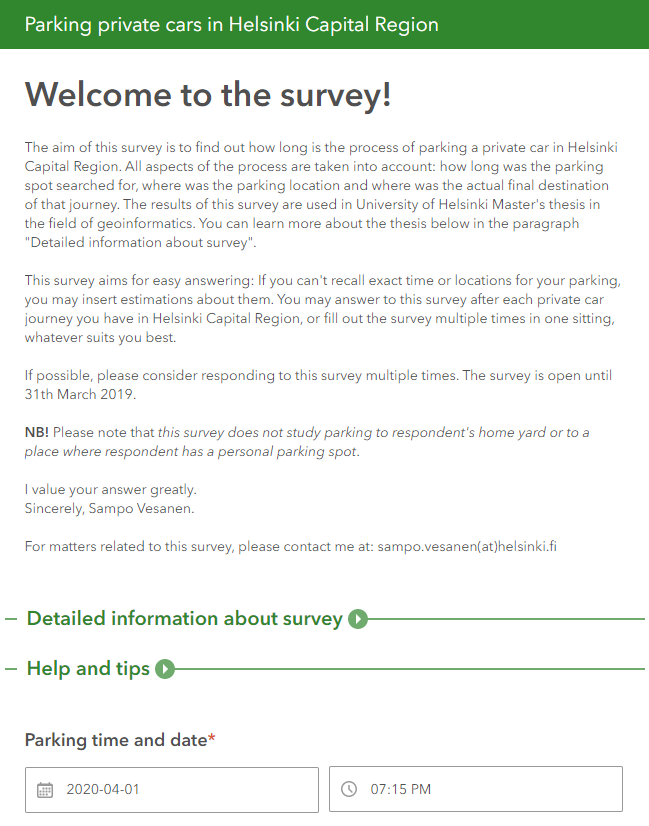
\includegraphics[width=5.5cm]{survey123_1.png} }}%
    \subfloat[Map panels for the parking location and the final destination.]{{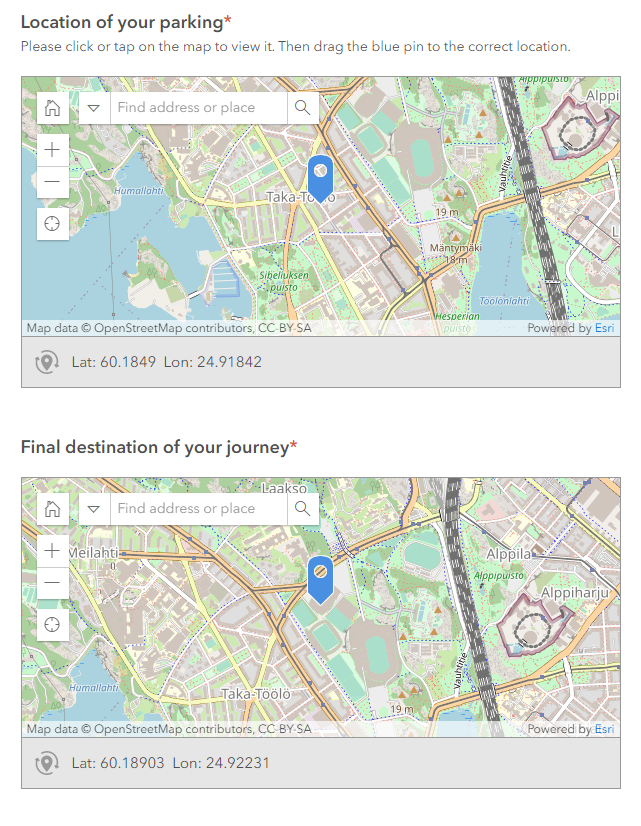
\includegraphics[width=5.5cm]{survey123_2.png} }}%
    \subfloat[Final questions of the survey.]{{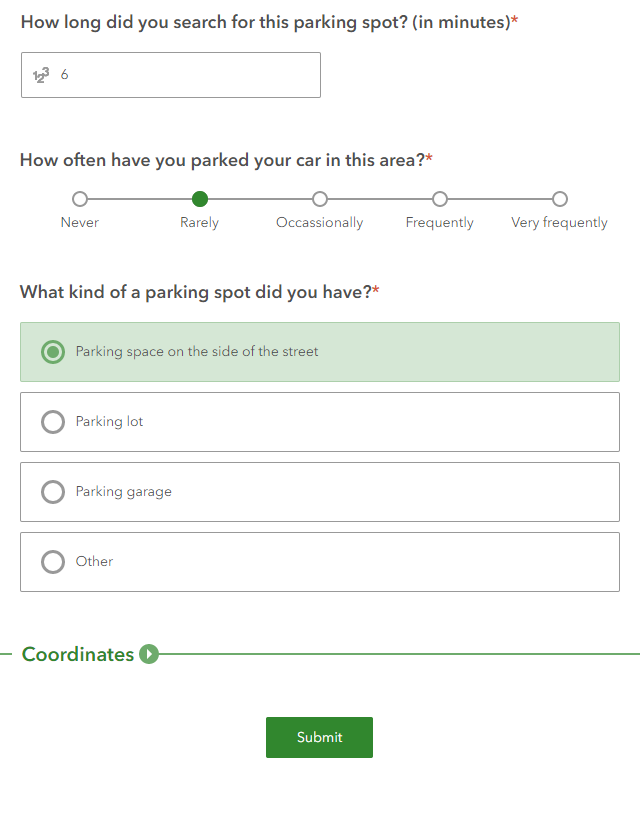
\includegraphics[width=5.5cm]{survey123_3.png} }}%
    \caption[The unused parking survey created with Survey123]{An example parking event entered into the parking research survey made with Survey123 Connect.}%
    \label{fig:survey123}%
\end{figure}

The survey was released even after Survey123 had proved itself unwieldly for the purposes of this research. The software was difficult to use because of an assortment of inconvenient design choices, unfinished functionality and a helping of software bugs. It was not possible, for example, to have respondents enter multiple parking events at once in a full screen map view. They would have to create a single parking event, send it, and then reload the survey to start from the beginning -- something a majority of prospective respondents would not have the patience for. Survey123 Connect version available at the time, 3.1.126, did not allow customisation of the post-submission message and therefore it would not be possible to efficiently direct respondents back to the form. In addition, recording coordinates from two map views was only possible through a bypass. The coordinates of the final destination would have to be printed on the form (hence the section "Coordinates" on the form in figure~\ref{fig:survey123}) and then these second set of coordinates could be saved into the survey data table in string format. The technical limitations of Survey123 as a spatial survey was witnessed also in the fact that it was not possible to add custom polygons on top of the map views. It was therefore impossible to delineate the research area for the respondents and accurately detect attempts to add parking events outside of Helsinki Capital Region.

The functionality of the released form was not reliable on the most popular web browsers such as Google Chrome and Apple Safari. Survey123 supported multi-language strings but it proved problematic to ensure that the form would open in the system language of most respondents, Finnish. In addition to this, the field for entering the specific time for the parking event was restricted to the 12 hour clock preferred in the US -- a system my target group would frown upon. To make matters worse, at that time there was a long persisting bug in Survey123 which produced unexpected behaviour, in some cases, with the use of "constraint", the parameter that controls which entered values are deemed illegal and which are not (\cite{GeoNet-TheEsriCommunity2018}). If any type of constraint statement was added, the finalised form would always claim that the related question input was invalid. The parameter would have to be left empty and therefore it was not possible to automatically prevent insertion of parking events happening in the future and excessively long times for searching for parking, reducing the quality of the survey data and making the survey form more confusing for the respondent.

\begin{figure}[H]%
    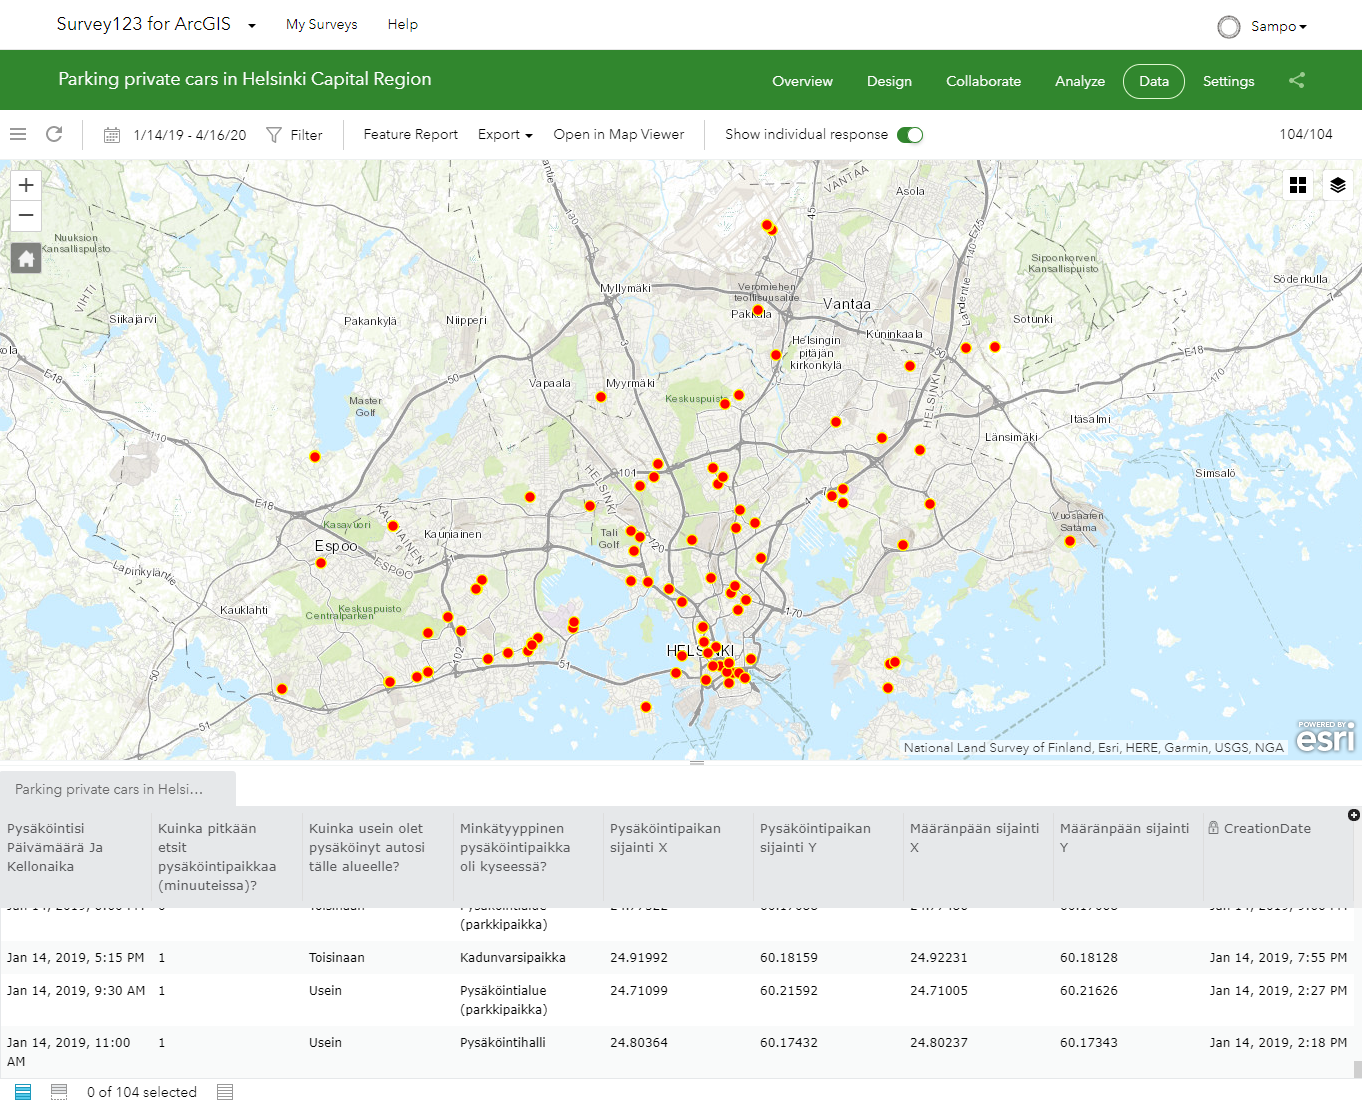
\includegraphics[width=\textwidth]{images/survey123_dataview.png}
    \caption[Survey123 data tab]{Survey123 for ArcGIS, "data" tab view in the application website. The research survey made with Survey123 received in total 104 parking events. The red dots are the final destinations of each parking event.}%
    \label{fig:survey123_dataview}%
\end{figure}

Despite the many technical incertainties of Survey123, the survey gathered more than one hundred parking events in one month (figure~\ref{fig:survey123_dataview}). This amount was achieved for the most part without advertising. Soon after the publication of the Survey123 parking survey it was decided, however, that the required spatial resolution for this research would need to be lower than exact points in an attempt to gather more responses from the entire research area. An additional deciding factor was the fact that with Survey123 respondents could not send multiple parking events with one survey session, making the form unwieldy and outdated in its rigid structure. It was argued that a more general scale would still be accurate enough to provide good data and a more generalised scale would make the survey easier to answer to and a more pleasant experience for the respondent. Postal code areas were deemed an acceptable compromise in spatial accuracy.

After careful consideration, it was decided that the survey for this thesis would have to be programmed from the ground up.

\subsubsection{Programming the parking survey}
\justify
To achieve maximum transparency and repeatability for this research, in addition to freedom in survey content and appearance, a survey web application was programmed from the ground up utilising HTML, JavaScript and PHP. The survey and its supporting infrastructure was installed on a virtual machine in CSC's -- the state owned ICT solutions company -- Taito supercluster. CSC offers virtual machines in several different hardware configurations, or flavors. The virtual machine flavor picked for this survey was \textit{standard.medium}, a flavor with 3.9 \gls{GB} \gls{RAM}, three virtual \gls{CPU}s and 80 GB of disk space. Running on the Linux distribution Ubuntu version 16.04, the backbone of the survey ecosystem was a LAMP stack, a software bundle which incorporates the Linux operating system, Apache web server software, \gls{mysql} relational database management system and the PHP programming language environment for server-side scripting. The public component of the survey is the front-end, the only component of the survey system a respondent would interact with (figure~\ref{fig:js_survey_welcome}). One may use additional software in a LAMP stack for extended functionality or can replace some of the components with a wide array of alternatives. This thesis utilises the components described in the table~\ref{tab:survey_components}.

\begin{hyphenrules}{nohyphenation}
    \begin{table}[H]
        \centering
        \def\arraystretch{1.2}
        \setlength\tabcolsep{1.2ex}
        \caption{Survey web application components} 
        \label{tab:survey_components}
        \begin{tabular}{ @{} >{\raggedright\arraybackslash}p{3cm} >{\raggedright\arraybackslash}p{3cm} >{\raggedright\arraybackslash}p{5.5cm} @{} }
            \toprule
            Component & Version & Description \\
            \midrule
            Ubuntu & 16.04.6 & Linux distribution, operating system for the virtual machine \\
            Apache HTTP Server & 2.4.18-2ubuntu3.9 & Web server software, manage website requests and responses \\
            MySQL & 5.7.25-0ubuntu0.16.04.2 & Relational database management system, survey database operations \\
            PHP & 7.0.33-0ubuntu0.16.04.1 & Programming language, used for server side scripting \\
            Parking survey front-end & 16.5.2019 & Survey visible to user, graphical user interface \\        
            \bottomrule
        \end{tabular}
    \end{table}
\end{hyphenrules}

Setting up the virtual machine for the use of the survey was a process of a few stages. The LAMP stack was installed on the fresh virtual machine with the command \code{sudo apt install lamp-server\^}. After the successful installation the MySQL tables were formed and relevant users created. The last step before a fully functioning web server was using root access to give the survey components permission to access relevant system directories. The parking survey's GitHub repository (\textcolor{blue}{\url{https://github.com/sampoves/parking-in-helsinki-region}}) may be viewed for the full step-by-step install procedure used to set up the web server for this thesis.

\begin{figure}[H]%
    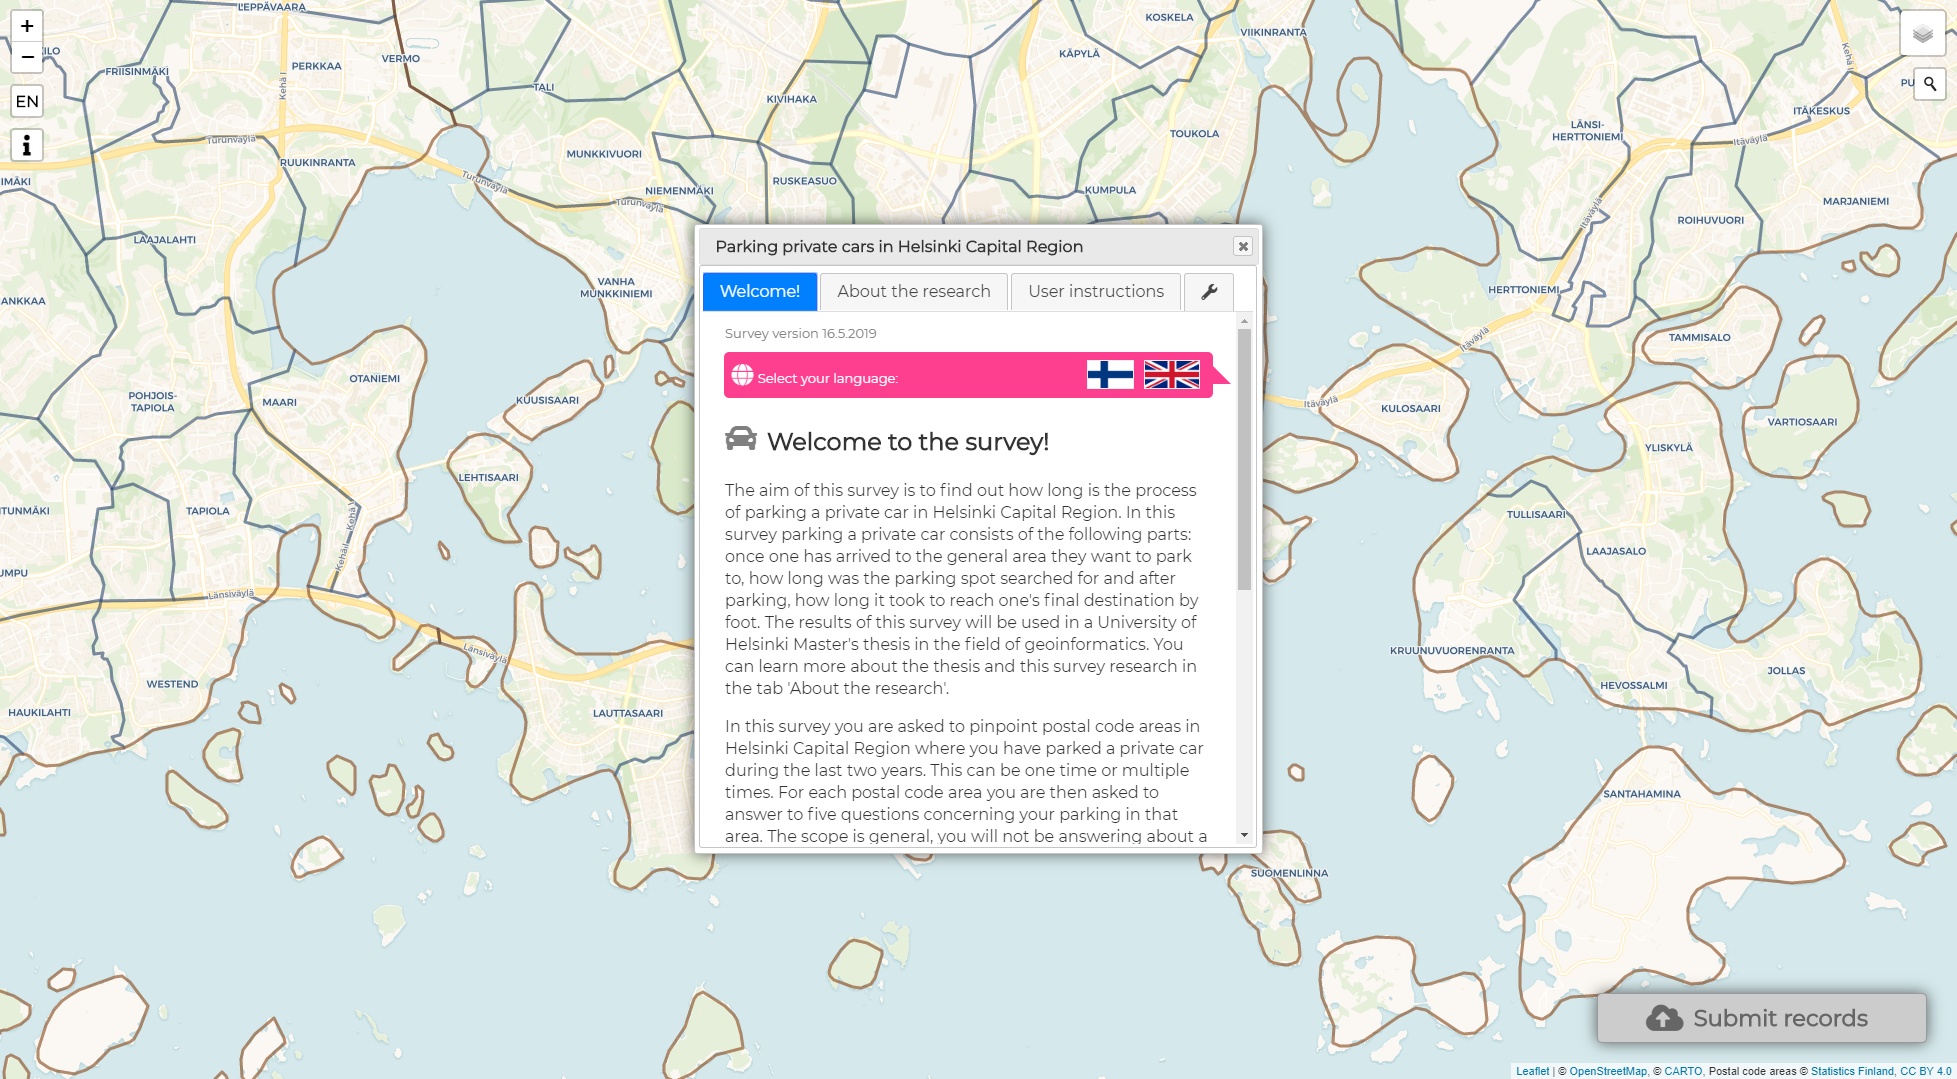
\includegraphics[width=\textwidth]{images/js_survey_welcome.png}
    \caption[Survey landing page]{The parking survey initial view with the welcoming dialog window.}%
    \label{fig:js_survey_welcome}%
\end{figure}

The survey front-end was programmed in NetBeans \gls{ide} 8.2 in mostly JavaScript using an open-source mapping library Leaflet (software version 1.4.0) in January--May 2019. In the survey, the respondent was presented with a map view of Helsinki Capital Region with its 167 postal code areas with the ability to drag the view, zoom in and out, search for places and addresses, choose the language between English and Finnish, and tweak various other settings to their liking. In this web survey, the respondent was asked to pick as many postal code areas as they could remember parking in in the last two years, and answer to five questions per each postal code area (table~\ref{tab:js_survey_questions} and figure~\ref{fig:js_survey_questions}). In each question, the respondent was asked to estimate their parking experience in that postal code area usually during the past two years. The last two years was chosen as the timeframe to allow respondents to comfortably recall parking events which happened during the subjective notion of "recent memory" while also forbidding the submission of out of date parking times. 

\textcolor{red}{lisää kappale, jossa selitän kysymysten sisällön auki, tsekkaa apu surveystä} The maximum values for searching for parking and walking to destination were consciously placed to 99 in an effort for the range to not feel restrictive for thes survey respondent.

In the introduction to the survey, it was explained to respondents that all answers were meant to be estimates as the survey was not about an exact time and place. To mitigate confusion and errors made by respondents a comprehensive help functionality and a location search tool were implemented in the parking survey. Once the respondent was finished with the survey, they would send their responses to the server. Respondents were welcomed to return to the survey to send additional data on any postal code areas they had missed the last time.

\begin{hyphenrules}{nohyphenation}
    \begin{table}[H]
        \centering
        \caption{Survey questions and question choices.} 
        \label{tab:js_survey_questions}
        \def\arraystretch{1.5}
        \setlength\tabcolsep{1.2ex}
        \begin{tabular}{ @{} >{\raggedright\arraybackslash}p{5.5cm} >{\raggedright\arraybackslash}p{5cm} >{\raggedright\arraybackslash}p{2.5cm} >{\raggedright\arraybackslash}p{2cm} @{} }
            \toprule
            Question & Question choices & Question type & Abbreviation \\
            \midrule
            How long does it usually take for you to find a parking spot and park your car in this postal code area (in minutes)? & 0--99 & Field, selection within range & parktime \\
            How long does it usually take for you to walk from your parking spot to your destination in this postal code area (in minutes)? & 0--99 & Field, selection within range & walktime \\
            How familiar are you with this postal code area? & 1 -- Extremely familiar\linebreak2 -- Moderately familiar\linebreak3 -- Somewhat familiar\linebreak4 -- Slightly familiar\linebreak5 -- Not at all familiar & Radio button group, likert-type scale & likert \\
            What kind of parking spot do you usually take in this postal code area? & 1 -- Parking space on the side of the street\linebreak2 -- Parking lot\linebreak3 -- Parking garage\linebreak4 -- Private or reserved spot\linebreak5 -- Other & Dropdown, selection & parkspot \\
            At what time of the day do you usually park in this postal code area? & 1 -- Weekday, rush hour (07.00--09.00 and 15.00--17.00)\linebreak2 -- Weekday, other than rush hour\linebreak3 -- Weekend\linebreak4 -- None of the above, no usual time & Dropdown, selection & timeofday \\
            \bottomrule
        \end{tabular}
    \end{table} 
\end{hyphenrules}

\begin{figure}[H]%
    \centering
    \subfloat[Survey questions in English.]{{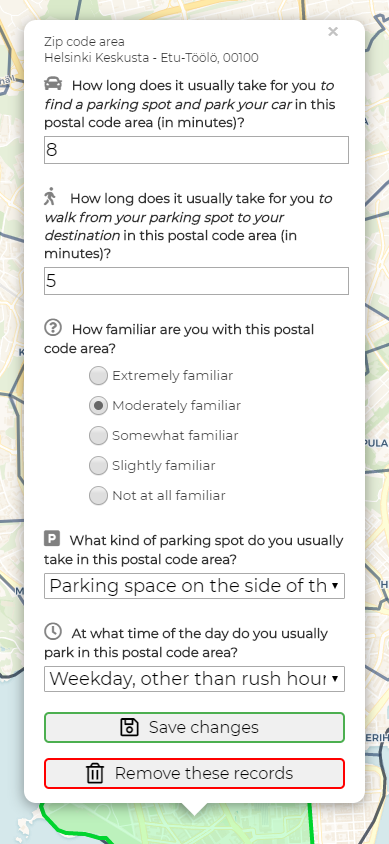
\includegraphics[width=6.25cm]{js_survey_en.png} }}%
    \qquad
    \subfloat[Survey questions in Finnish.]{{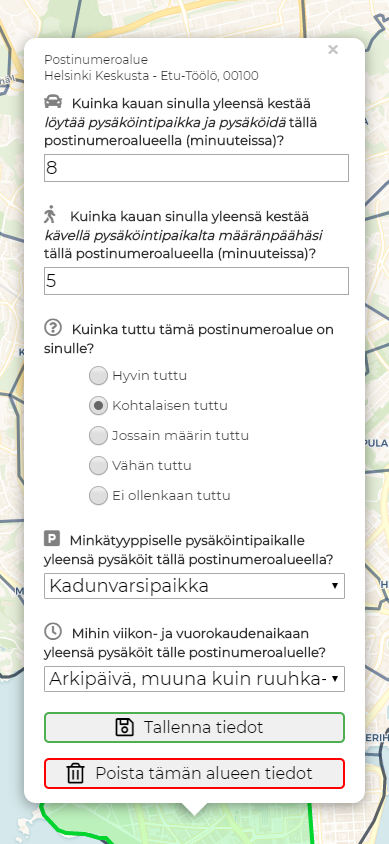
\includegraphics[width=6.25cm]{js_survey_fi.png} }}%
    \caption[Research survey questions in the web application]{For each postal code area of their choosing the respondent would answer to these five questions. The survey was made available in English and Finnish.}%
    \label{fig:js_survey_questions}%
\end{figure}

When data was received from the respondent, a script written in \gls{php} verified the data contents. This was an effort to prevent attacks on the web server running the study survey. Only specific variables of specific types were accepted from the front-end. Additionally, the \gls{php} verification made sure falsified or incomplete data would not be accepted into the database containing the verified results. If the server-side verification test failed in any way, the respondent was informed about it. 

In addition to the data verification, a PHP script tracked the IP addresses which accessed the survey web server. By using the survey, respondents agreed that their IP addresses were recorded for the use of this thesis solely to identify falsified or overlapping data and detect unique visits. All IP addresses were anonymised with a Python script and original sensitive data deleted. The anonymisation script is available for viewing at the thesis data analysis repository at GitHub (\textcolor{blue}{\url{https://github.com/sampoves/Msc-thesis-data-analysis}}).

As a final survey component, the server side contained two MySQL datatables, one for received data (table~\ref{tab:mysql_records}) and another for survey web page hits (table~\ref{tab:mysql_visitors}). In the table \textit{records}, the following data was recorded: time of sending (column name \code{timestamp}), IP address (\code{ip}), postal area code (\code{zipcode}), a value in the sequence 1--5 for the likert question (\code{likert}), a value in the sequence 1--5 for the question what type of parking spot was used (\code{parkspot}), an integer value for how long it usually took to park in this location (\code{parktime}), an integer value for how long it usually took to walk from parking place to one's destination (\code{walktime}), and a value in the sequence 1--4 for the question at what time of the day one usually parks in the location (\code{timeofday}) (table~\ref{tab:mysql_records_str}). In the table \textit{records}, it is notable that in the case an respondent sent the web server data for multiple postal code areas each of the postal code areas would take up their own row in the data table. Consequently, it was theoretically possible for one respondent to simultaneously submit 167 rows of data.

In the table \textit{visitors}, the following data was recorded: IP address (\code{ip}), the timestamp of the first visit of this IP address (\code{ts\_first}), the timestamp of latest visit of this IP address (\code{ts\_latest}), and the count of visits (\code{count}). In this table, an IP address is only stored once. On the first visit of an IP address, the row for that IP address is created in the data table with \code{ts\_first} and \code{ts\_latest} being identical. On further visits of that IP address the original row is appended with updated information in the columns \code{ts\_latest} and \code{count} (table~\ref{tab:mysql_visitors_str}).

\begin{hyphenrules}{nohyphenation}
    \begin{table}[H]
        \centering
        \setlength\tabcolsep{1.2ex}
        \caption[Structure of MySQL table records]{The structure of the survey MySQL table \textit{records} fetched with the statement \code{DESCRIBE records;}} 
        \label{tab:mysql_records_str}
        \begin{tabular}{ @{} >{\raggedright\arraybackslash}p{2cm} >{\raggedright\arraybackslash}p{2cm} >{\raggedright\arraybackslash}p{1cm} >{\raggedright\arraybackslash}p{1cm} >{\raggedright\arraybackslash}p{1.5cm} >{\raggedleft\arraybackslash}p{4cm} @{} }
            \toprule
            Field & Type & Null & Key & Default & Extra \\
            \midrule
            id & int(11) & No & PRI & NULL & AUTO\_INCREMENT \\
            timestamp & varchar(19) & Yes & & NULL & \\
            ip & TEXT & Yes & & NULL & \\
            zipcode & varchar(5) & Yes & & NULL & \\
            likert & int(1) & Yes & & NULL & \\
            parkspot & int(1) & Yes & & NULL & \\
            parktime & int(2) & Yes & & NULL & \\
            walktime & int(2) & Yes & & NULL & \\
            timeofday & int(1) & Yes & & NULL & \\
            \bottomrule
        \end{tabular}
    \end{table} 
\end{hyphenrules}

\begin{hyphenrules}{nohyphenation}
    \begin{table}[H]
        \centering
        \setlength\tabcolsep{1.2ex}
        \caption[Structure of MySQL table visitors]{The structure of the survey MySQL table \textit{visitors} fetched with the statement \code{DESCRIBE visitors;}} 
        \label{tab:mysql_visitors_str}
        \begin{tabular}{ @{} >{\raggedright\arraybackslash}p{2cm} >{\raggedright\arraybackslash}p{2cm} >{\raggedright\arraybackslash}p{1cm} >{\raggedright\arraybackslash}p{1cm} >{\raggedright\arraybackslash}p{1.5cm} >{\raggedleft\arraybackslash}p{4cm} @{} }
            \toprule
            Field & Type & Null & Key & Default & Extra \\
            \midrule
            id & int(11) & No & PRI & NULL & AUTO\_INCREMENT \\
            ip & TEXT & Yes & & NULL & \\
            ts\_first & DATETIME & Yes & & NULL & \\
            ts\_latest & DATETIME & Yes & & NULL & \\
            count & int(11) & Yes & & NULL & \\        
            \bottomrule
        \end{tabular}
    \end{table} 
\end{hyphenrules}

The parking survey was released to the public in May 2019 and the active phase of collecting data continued until 30th June 2019. However, the survey remained open after thiss active period, receiving the last row of data in October 2019. The majority of the respondents were found through Facebook. Invitations to participate in the survey were sent to 112 city district and neighborhood groups with a theoretical reach of tens of thousands of people. Of the 112 posts, 63 were Helsinki centric groups, while 22 were from Espoo, 15 from Vantaa, and 12 from municipalities bordering Helsinki Capital Region. In addition to these city district and municipal groups, invitation to participate was sent to two other Facebook groups, "Lisää kaupunkia Helsinkiin", a group for city planning ethusiasts in Helsinki, and the GIS profession group "GIS-velhot". It is not possible to conclusively differentiate from which group or city survey data originated from. A clue about the survey's popularity in each city, however, may be gained from the table \textit{visitors} due to the fact that invitation posts were sent over multiple days to the groups in the order: 

\begin{displayquote}
$\text{Espoo}\rightarrow\text{Helsinki}\rightarrow\text{Vantaa}\rightarrow\text{bordering municipalities}\rightarrow\text{reminders to the largest groups}$
\end{displayquote}

In addition to Facebook, an effort was also made to get faculty members of geosciences and geography and students of University of Helsinki to participate in the survey. A small amount of answers were collected with a tweet sent from the Twitter account of Digital Geography Lab. After the initial invitation to participate, reminders were sent to the largest Facebook groups one month after the original posts.

The source code for the survey described in this chapter and step-by-step information to set up an identical system is available at GitHub (\textcolor{blue}{\url{https://github.com/sampoves/parking-in-helsinki-region}}). As a side product, a variant of this survey was created where respondents pick precise points instead of areas. This point-based survey template is, too, available at GitHub (\textcolor{blue}{\url{https://github.com/sampoves/leaflet-map-survey-point}}). The parking survey web application as it was used in this thesis may be tested in the following web address: \textcolor{blue}{\url{https://parking-survey.socialsawblade.fi}}.

% \scalebox to prevent table going too wide
\begin{hyphenrules}{nohyphenation}
    \begin{table}[H]
        \centering
        \setlength\tabcolsep{2pt}
        \caption[MySQL table records]{An excerpt of the data content of the research survey MySQL table \textit{records}.} 
        \label{tab:mysql_records}
        \scalebox{0.9}
        {\begin{tabular}{ @{} >{\raggedright\arraybackslash}p{1.5cm} >{\raggedright\arraybackslash}p{4cm} >{\raggedright\arraybackslash}p{2.5cm} >{\raggedright\arraybackslash}p{2cm} >{\raggedright\arraybackslash}p{1.5cm} >{\raggedright\arraybackslash}p{1.5cm} >{\raggedright\arraybackslash}p{1.5cm} >{\raggedright\arraybackslash}p{1.5cm} >{\raggedright\arraybackslash}p{1.5cm} @{} }
            \toprule
            id & timestamp & ip & zipcode & likert & parkspot & parktime & walktime & timeofday \\
            \midrule
            3245 & 2019-06-06 21:41:21 & wro4qo8hv4 & 00510 & 1 & 4 & 0 & 3 & 1 \\
            3246 & 2019-06-06 21:41:54 & aonm72lyx3 & 00520 & 2 & 1 & 10 & 5 & 1 \\
            3247 & 2019-06-06 21:46:19 & n1982i4i2v & 00100 & 1 & 1 & 20 & 4 & 1 \\
            3248 & 2019-06-06 21:46:22 & sbhfz0uvsl & 00210 & 1 & 1 & 5 & 3 & 3 \\
            3249 & 2019-06-06 21:46:22 & sbhfz0uvsl & 00220 & 2 & 2 & 5 & 5 & 2 \\        
            \bottomrule
        \end{tabular}}
    \end{table} 
\end{hyphenrules}

\begin{hyphenrules}{nohyphenation}
    \begin{table}[H]
        \centering
        \setlength\tabcolsep{1pt}
        \caption[MySQL table visitors]{An excerpt of the data content of the research survey MySQL table \textit{visitors}.} 
        \label{tab:mysql_visitors}
        \begin{tabular}{ @{} >{\raggedright\arraybackslash}p{2cm} >{\raggedright\arraybackslash}p{3cm} >{\raggedright\arraybackslash}p{4cm} >{\raggedright\arraybackslash}p{4cm} >{\raggedleft\arraybackslash}p{1cm} @{} }
            \toprule
            id & ip & ts\_first & ts\_latest & count \\
            \midrule
            1780 & mvovd467a7 & 2019-05-26 15:25:23 & 2019-05-26 15:26:06 & 2 \\
            1781 & xgbgkkzxb3 & 2019-05-26 15:26:23 & 2019-05-26 15:26:23 & 1 \\
            1782 & c9qer4q99a & 2019-05-26 15:27:25 & 2019-05-26 15:27:25 & 1 \\
            1783 & cujhd0hng7 & 2019-05-26 15:27:29 & 2019-05-26 15:27:29 & 1 \\
            1784 & 3ja7gjtko6 & 2019-05-26 15:28:45 & 2019-05-26 15:29:20 & 2 \\        
            \bottomrule
        \end{tabular}
    \end{table} 
\end{hyphenrules}

\begin{figure}[H]%
    \centering
    \subfloat[Respondent arrives to the survey web application to see a map with the postal code areas of Helsinki Capital Region lined out.]{{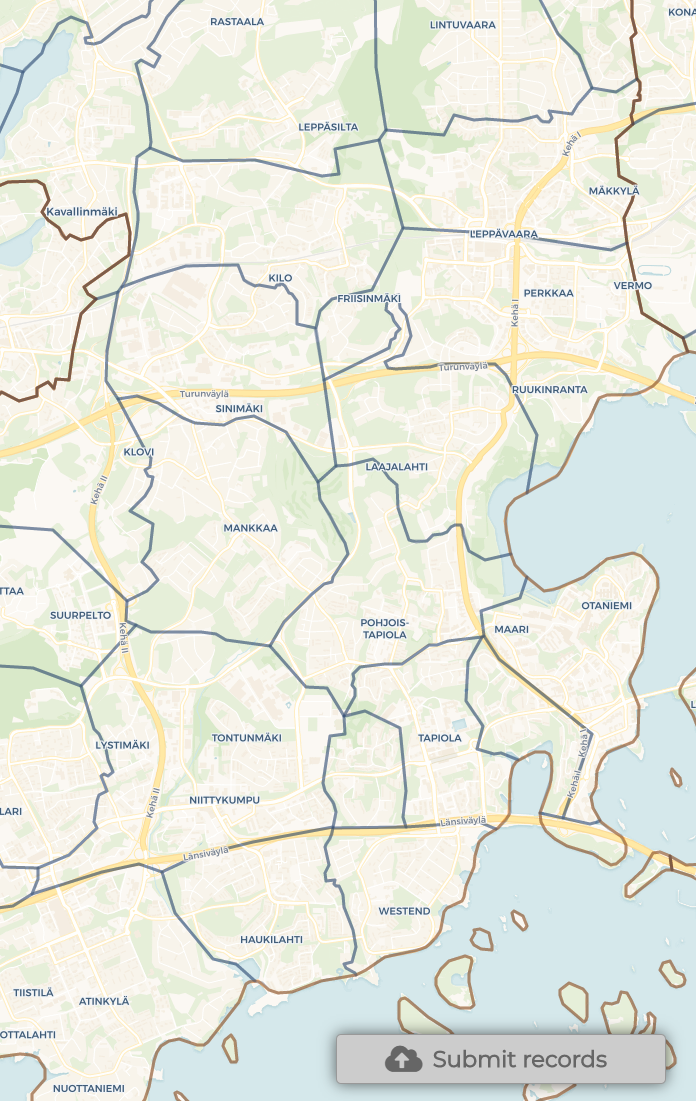
\includegraphics[width=7cm]{js_survey_process1.png} }}%
    \quad
    \subfloat[Respodent proceeds to fill out their parking experiences in freely chosen postal code areas.]{{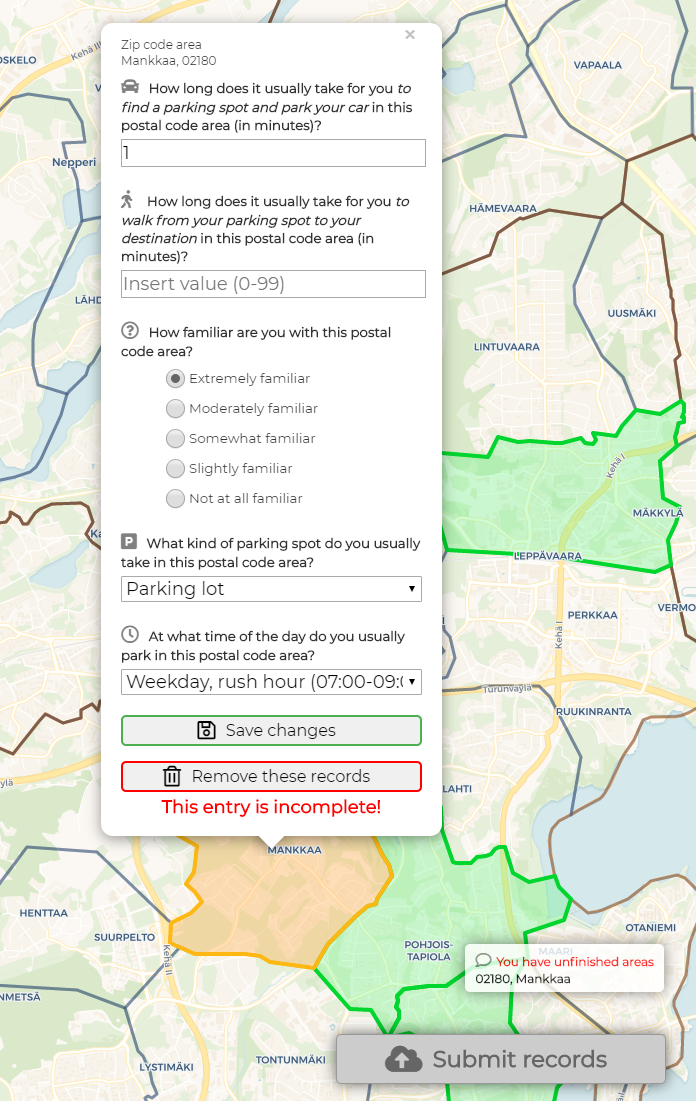
\includegraphics[width=7cm]{js_survey_process2.png} }}%
    \quad
    \subfloat[\textit{Submit records} button activates when all questions in all selected postal code areas are completed.]{{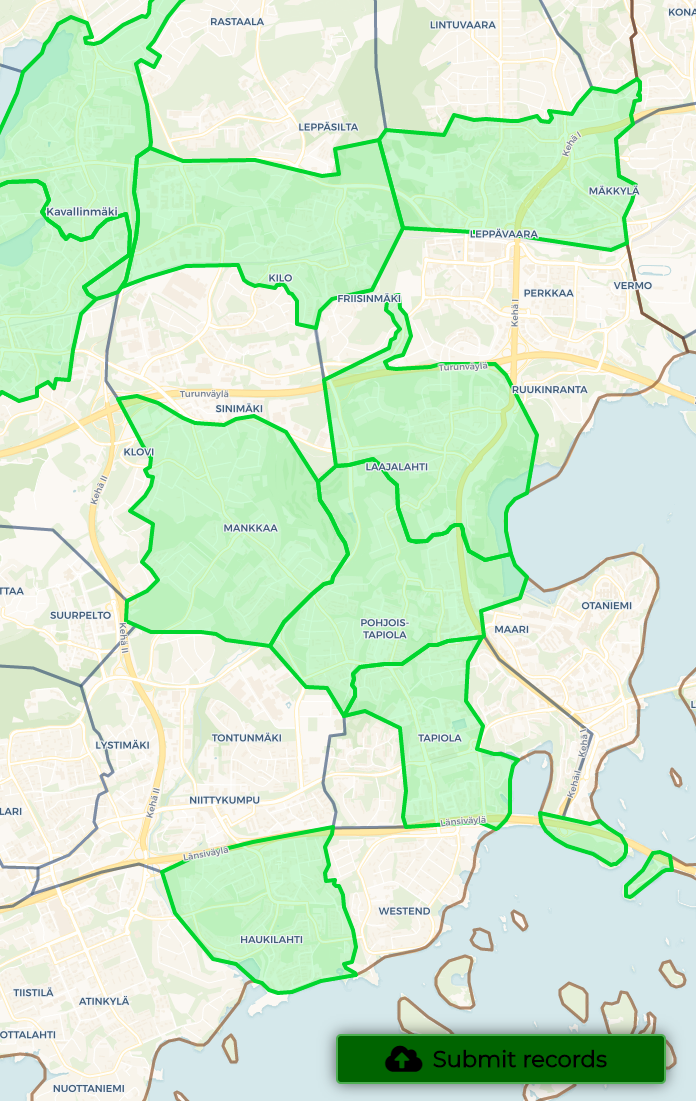
\includegraphics[width=7cm]{js_survey_process3.png} }}%
    \quad
    \subfloat[Respondent receives a prompt to confirm that their submission was successful.]{{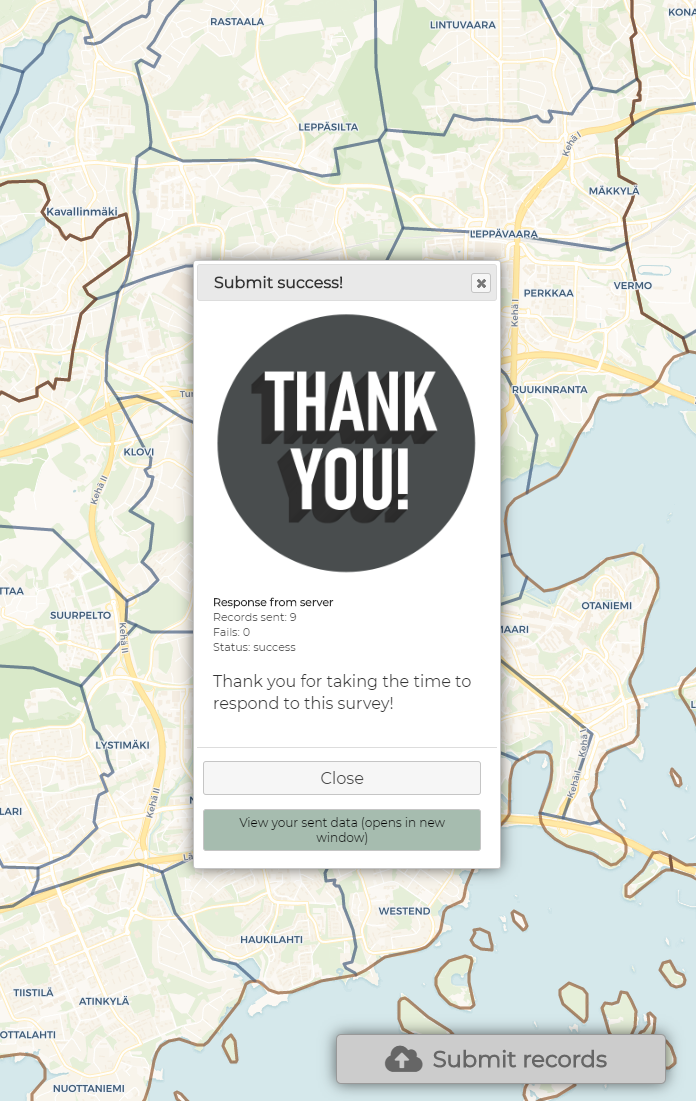
\includegraphics[width=7cm]{js_survey_process4.png} }}%
    \caption[Steps to fill out the survey]{A respondent would follow these steps to submit data through the survey web application.}%
    \label{fig:survey_process}%
\end{figure}

\newpage
\subsection{Processing survey data}
\label{sec:processdata} % labeling to enable hyperref to this chapter
\justify
%\begin{itemize} %processingin tärkeimmät kohdat
%    \item anonymisation of ip addresses
%    \item Read in spatial data sources
%    \item Read in survey data
%    \item Prepare source data (convert formats, remove some irregular erroneous answers from dataset)
%    \item Prepare shape files (remove islands not reachable by car)
%    \item give grid cells zipcodes (ykr grid does not have those of-the-shelf. Develop method to assign all cells zipcodes, take into account water and grid cells which are outside of research area)
%    \item respondent behaviour (see how each user has answered)
%    \item detect illegal data (first detect duplicate answers, produce report. Then remove data where parktime and/or walktime is 60 or over)
%    \item Add data to geodataframes (add columns for ykr\_vyoh, ua-forest, answer count, parktime and walktime mean
%    \item show statistics to user
%    \item Set percentage of urban zones and forest in each zipcode area (choose one urban zone and forest amount (jenks breaks) for every zipcode)
%    \item add subdivisions to data (all answer row gets corresponding subdivision value)
%    \item EXPERIMENTAL utilise travel-time matrix 2018, make comparisons
%    \item EXPERIMENTAL somehow create my own TTM18, with updated values
%    \item export results to R
%\end{itemize}

In this section, various data are refered to with abbreviated names as this makes it easier to follow the data processing workflow. Please see table~\ref{tab:used_data} for the key. \textcolor{red}{kaikki kohdat tässä kappaleessa ei käytä lyhenteitä (records, visitors, postal)}

The main objective of the thesis data processing was to merge survey responses (\textit{records}) with selected spatial data and prepare \textit{records}, survey visits (\textit{visitors}), \textit{postal}, and \textit{grid} for later analysis in R programming language environment. Using a selection of open spatial data (table~\ref{tab:used_data}), new explanatory variables would be available for use in the analysis. This opened opportunities to compare the newly gathered survey data against that in Helsinki Travel-time Matrix 2018. \textcolor{red}{toistoa} \textcolor{purple}{All data processing in this phase was carried out in Python programming language version 3.7.6, using Anaconda, a free and open-source Python distribution for scientific programming. Anaconda version 2020.02 included all essential packages for carrying out the script, with the exception of GeoPandas 0.5.0, the package for geospatial data manipulation in Python. GeoPandas and its dependencies -- GDAL 2.4.1, Fiona 1.8.6, pyproj 2.1.3, rtree 0.8.3, and Shapely 1.6.4.post1 -- were manually installed through Python package installer pip (table~\ref{tab:used_soft})}.

As the first step in the survey data processing, all IP addresses were anonymised and replaced with identifiers of ten characters consisting of numbers 0--9 and letters of English alphabet (figure~\ref{fig:gen_workflow}, section 1). The anonymisation was carried out in such a way that the random identifiers for respondents matched in both \textit{records} and \textit{visitors}, preserving the possibility to associate survey responses with survey visits. 

\begin{figure}[H]%
    \centering
    \subfloat[Unedited PAAVO postal code areas for Helsinki Capital Region.]{{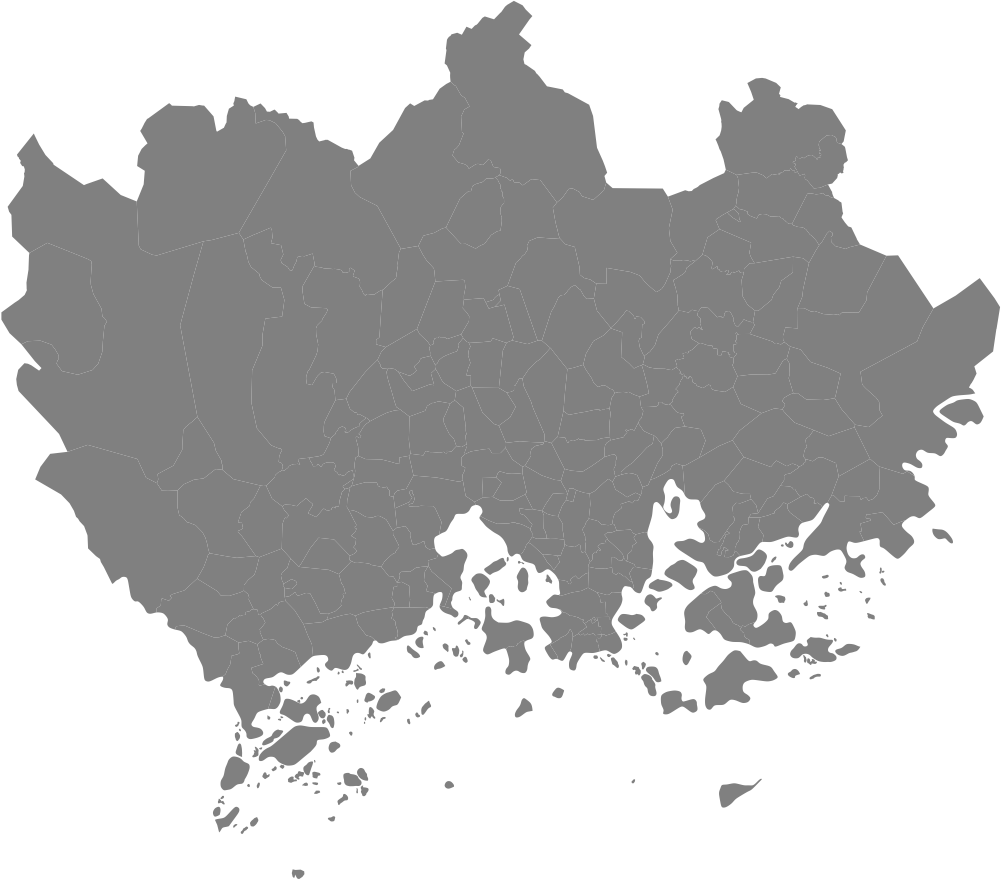
\includegraphics[width=8.1cm]{resarea_unedited.png} }}%
    \quad
    \subfloat[PAAVO postal code areas for Helsinki Capital Region, islands unreachable by car removed.]{{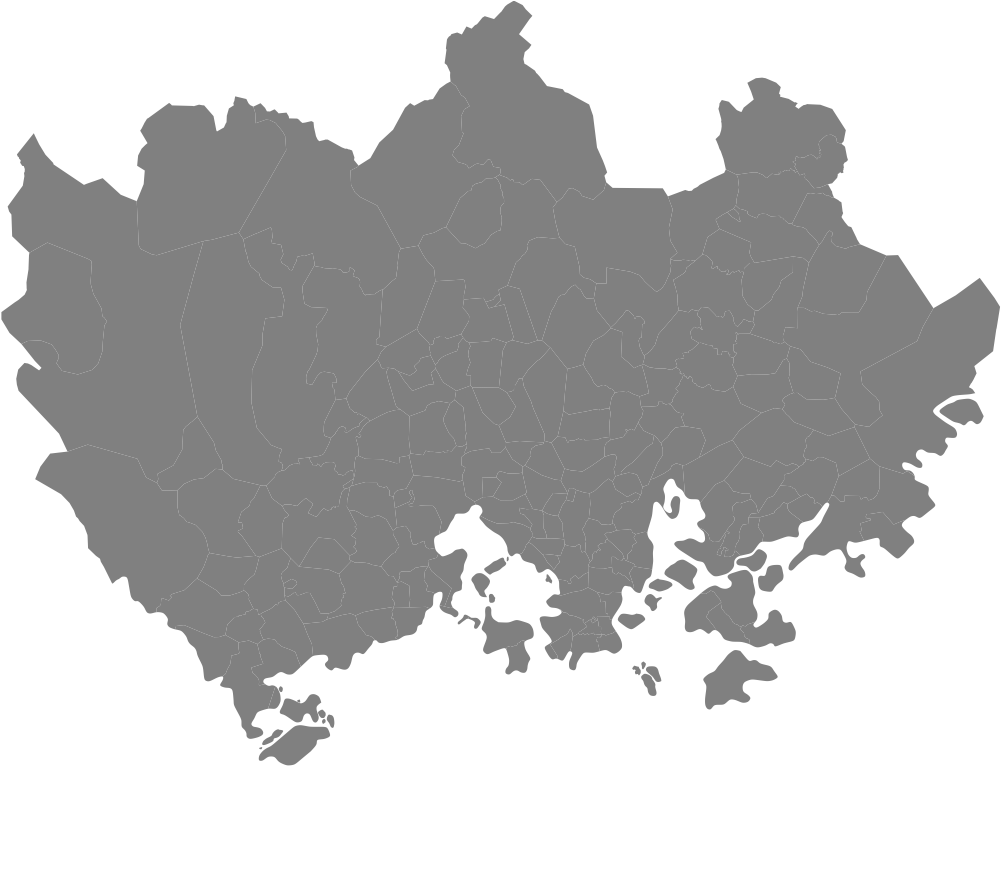
\includegraphics[width=8.1cm]{resarea_edited.png} }}%
    \caption[Process to remove islands not reachable by car]{Islands unreachable by car were removed from the postal code area data in the Python data processing.}%
    \label{fig:paavo_resarea}%
\end{figure}

The data processing proper started with loading the open spatial data presented in table~\ref{tab:used_data} and selecting only areas relevant to the research (figure~\ref{fig:gen_workflow}, section 2). For \textit{CORINE}, this meant selecting only areas marked Level1Eng, Artificial surfaces. \textit{YKR zones}, a dataset that covers the entirety of Finland, was clipped with spatial dimensions of PAAVO postal code areas data, \textit{postal}, that had been extended with a 500 meter buffer. \textit{postal} was processed to only include areas reachable by car from the mainland (figure~\ref{fig:paavo_resarea}). Islands not reachable by car were approximated visually using Google Maps and were removed from the data. However, some islands in Helsinki Capital Region are technically accessible with a car from the mainland, but in practice the access is limited. In these cases, deliberation was used. For example, Suomenlinna islands and Korkeasaari were kept in the data. Conversely, some technically car-accessible islands like Staffan in Espoo, and Mustasaari and Seurasaari in Helsinki were removed from the data with the grounds of them containing only private property, or no public parking spaces. \textcolor{red}{selitä laajemmin miksi näitä saaria poistellaan (analyysi ja visualisointi). lisäksi, mieti toi logiikka "yksityisalue tai ei yleisiä parkkiksia"}

\begin{figure}[H]%
    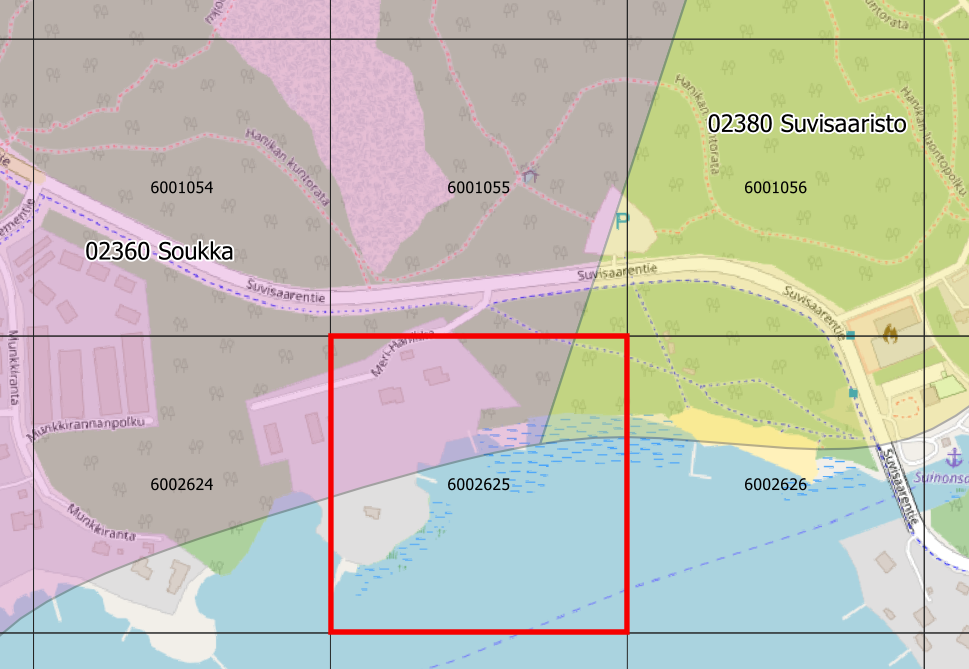
\includegraphics[width=\textwidth]{images/paavo-ykr.png}
    \caption[Assigning MetropAccess-YKR-grid postal codes]{The MetropAccess-YKR-grid cell 6002625 (marked with the red square) is assigned postal code 02360 because in that grid cell, the largest segment of PAAVO open data (coloured warm purple and yellow) belongs in the postal code 02360 Soukka. \textcolor{red}{osm cite}}%
    \label{fig:paavo_ykr}%
\end{figure}

Helsinki Region Travel Time Matrix 2018 and the survey data of this thesis operate in different spatial units. Travel time Matrix 2018 uses the MetropAccess-YKR-grid (\textit{grid}), a spatial dataset based on the Statistics Finland statistical grid with the cell size of 250 x 250 meters. The basic spatial unit of the survey data is the postal code area based on PAAVO open data (\textcolor{red}{lisää lähteet}). Using Python, postal codes were added to each \textit{grid} cell with the logic that the largest area in \textit{postal} (figure~\ref{fig:paavo_ykr}) assigns the postal code in each \textit{grid} cell. \textit{postal} polygons do not always intersect with the cells of \textit{grid} and because of this some cells were assigned a postal code of 99999 to denote missing data (\textcolor{red}{mieti vielä 99999:n käyttö}). As a side product of this postal code assignment, \textit{grid} was merged with data which tells how much of a cell was contained in the research area (\textit{postal}) and how large was the largest postal code area which dictated the postal code assignment of the current cell. \textcolor{red}{varmista että lukija ymmärtää PAAVO spatial datan ja tutkimusalueen yhteyden}

The data processing script created for this thesis contains detailed features to detect patterns in the survey data (figure~\ref{fig:gen_workflow}, section 3). To enhance pattern recognition, \textit{records} and \textit{visitors} were purged of known false data, which were namely responses and visits made by me.

The data processing script creates two distinct reports about \textit{records}. Firstly, the data processing script aggregates \textit{records} by IP address code, resulting in an Excel file where one row represents each respondent. It is then possible to review the behaviour of each respondent in detail. In addition to this report, the data processing script writes a text file report about IP address codes which submitted multiple responses from the same postal code area. The text file report also identifies whether the duplicate responses for each postal code area per each IP address code have identical values or if they have changed between responses. These two reports were used to determine what to do about the duplicates and values which appear anomalous.

It was decided that if the parking time or walking time value in a \textit{records} row was 60 minutes or greater, that data row would be deleted. This value is arbitrary. The research assumes that it is highly unlikely that anybody would generally park 60 minutes away from their final destination to which they would then proceed on foot. A hour of searching for parking is plausible in the center of Helsinki but because of its unlikeliness the same 60 minutes limit was utilised in searching for parking. It is not possible to determine why multiple survey responses contain the maximum value for parktime and walktime, 99, but it can not be ruled out that these data rows are protest votes meant to declare that reliable parking is hard to find in certain parts of Helsinki Capital Region. When advertising the thesis survey on Facebook, some people took the opportunity to voice their displeasure at the perceivedly difficult parking conditions in the Helsinki Capital Region. In conclusion, even though the Python script has the capability to delete data rows deemed illegal, all of the illegal data in \textit{records} was preserved a more versatile analysis in R.

Next in the survey data processing workflow the additional spatial data was added to \textit{postal}, the dataset with one row for each postal code area (figure~\ref{fig:gen_workflow}, section 4). Utilising \textit{records}, functions \code{sum}, \code{mean}, and \code{median} were used to produce answer count, and means and medians for parktime and walktime for all postal code areas. Each postal code area also received seven columns to depict the share of \textit{YKR zones} classes in percentage. It must be noted that before applying the \textit{YKR zones} data to the thesis data, classification in the source data was simplified with following the notation presented by the research group at the websites of the zones of urban structure (table~\ref{tab:ykr_zones_simplify}, \cite{FinnishEnvironmentInstitute2013}). Using \textit{CORINE} data, the percentage of artificial surface in each postal code area was calculated (table~\ref{tab:corine_artificial}).

\begin{hyphenrules}{nohyphenation}
    \begin{table}[H]
        \centering
        \def\arraystretch{1.2}
        \setlength\tabcolsep{1.2ex}
        \caption[YKR zones processing]{The logic by which the unedited source data for zones of urban structure was transformed for this thesis.}
        \label{tab:ykr_zones_simplify}
        \scalebox{0.9}
        {\begin{tabular}{ @{} >{\raggedright\arraybackslash}p{6cm} >{\raggedright\arraybackslash}p{6cm} @{} }
            \toprule
            Original definition & Definition for this thesis \\
            \midrule
            Keskustan jalankulkuvyöhyke & Keskustan jalankulkuvyöhyke \\
            \greyrule
            % Manually set the position of multirow label
            Keskustan reunavyöhyke & \multirow{3}{*}[-4.5ex]{Keskustan reunavyöhyke} \\
            Keskustan reunavyöhyke/intensiivinen joukkoliikenne & \\
            Keskustan reunavyöhyke/joukkoliikenne & \\
            \greyrule
            Alakeskuksen jalankulkuvyöhyke & \multirow{3}{*}[-4.5ex]{Alakeskuksen jalankulkuvyöhyke} \\
            Alakeskuksen jalankulkuvyöhyke/intensiivinen joukkoliikenne & \\
            Alakeskuksen jalankulkuvyöhyke/joukkoliikenne & \\
            \greyrule
            Intensiivinen joukkoliikennevyöhyke & Intensiivinen joukkoliikennevyöhyke \\ 
            \greyrule
            Joukkoliikennevyöhyke & Joukkoliikennevyöhyke \\
            \greyrule
            Autovyöhyke & Autovyöhyke \\
            \greyrule
            \textit{Areas not in the YKR zones data} & novalue \\
            \bottomrule
        \end{tabular}}
    \end{table} 
\end{hyphenrules}

\begin{hyphenrules}{nohyphenation}
    \begin{table}[H]
        \centering
        \def\arraystretch{1.2}
        \setlength\tabcolsep{1.2ex}
        \caption[CORINE data levels]{CORINE land cover 2018 data hierarchy under attribute data column Level1Eng, Artificial surfaces.}
        \label{tab:corine_artificial}
        \scalebox{0.85}
        {\begin{tabular}{ @{} >{\raggedright\arraybackslash}p{4cm} @{} >{\raggedright\arraybackslash}p{4cm} @{} >{\raggedright\arraybackslash}p{4.25cm} @{} >{\raggedright\arraybackslash}p{4cm} @{} }
            \toprule
            Level1, Level1Eng & Level2, Level2Eng & Level3, Level3Eng & Level4, Level4Eng \\
            \midrule
            \multirow{16}{4cm}[-15ex]{1 Artificial surfaces} & \multirow{2}{4cm}[-4ex]{11 Urban fabric} & 111 Continuous urban fabric 
 & 1111 Continuous urban fabric \\
            \arrayrulecolor{black!30}\cmidrule(lr){3-4}
            & & 112 Discontinuous urban fabric & 1121 Discontinuous urban fabric \\
            \arrayrulecolor{black!30}\cmidrule(lr){2-4}
            & \multirow{2}{4cm}[-0.5ex]{12 Urban fabric} & \multirow{2}{4cm}{121 Industrial or commercial units} & 1211 Commercial units \\
            \arrayrulecolor{black!30}\cmidrule(lr){4-4}
            & & & 1212 Industrial units \\
            \arrayrulecolor{black!30}\cmidrule(lr){2-4}
            & \multirow{3}{4cm}[-4ex]{12 Industrial, commercial and transport units} & 122 Road and rail networks and associated land & 1221 Road and rail networks and associated land \\
            \arrayrulecolor{black!30}\cmidrule(lr){3-4}
            & & 123 Port areas & 1231 Port areas \\
            \arrayrulecolor{black!30}\cmidrule(lr){3-4}
            & & 124 Airports & 1241 Airports \\
            \arrayrulecolor{black!30}\cmidrule(lr){2-4}
            & \multirow{4}{4cm}[-4ex]{13 Mine, dump and construction sites} & \multirow{2}{4cm}[-2.5ex]{131 Mineral extraction sites} & 1311 Mineral extraction sites \\
            \arrayrulecolor{black!30}\cmidrule(lr){4-4}
            & & & 1312 Open cast mines \\
            \arrayrulecolor{black!30}\cmidrule(lr){3-4}
            & & 132 Dump sites & 1321 Dump sites \\
            \arrayrulecolor{black!30}\cmidrule(lr){3-4}
            & & 133 Construction sites & 1331 Construction sites \\
            \arrayrulecolor{black!30}\cmidrule(lr){2-4}
            & \multirow{5}{4cm}[-2ex]{14 Artificial, non-agricultural vegetated areas} & 141 Green urban areas & 1411 Green urban areas \\
            \arrayrulecolor{black!30}\cmidrule(lr){3-4}
            & & \multirow{4}{4cm}[-3ex]{142 Sport and leisure facilities} & 1421 Summer cottages \\
            \arrayrulecolor{black!30}\cmidrule(lr){4-4}
            & & & 1422 Sport and leisure areas \\
            \arrayrulecolor{black!30}\cmidrule(lr){4-4}
            & & & 1423 Golf courses \\
            \arrayrulecolor{black!30}\cmidrule(lr){4-4}
            & & & 1424 Race courses \\
            \bottomrule
        \end{tabular}}
    \end{table} 
\end{hyphenrules}

% https://www.spatialanalysisonline.com/HTML/index.html?classification_and_clustering.htm
In the finalising section, \textit{records} was prepared for analysis and visualisation in R (figure~\ref{fig:gen_workflow}, section 5). The software library for plotting in R, \textit{ggplot2}, prefers data inputted in long format. To study charasteristics of postal code areas in this research, it meant adding repetitive data columns in \textit{records}, where values for CORINE land cover 2018 artificial surfaces, YKR zone and subdivision remained unchanged for all rows in the same postal code area. For artificial surfaces, a custom Jenks natural breaks function (GitHub user Drewda, \textcolor{red}{add cite, add jenks cite, kato kommenttilinkki}) with five classes were utilised to find the applicable Jenks breaks class for each postal code area. For YKR zones, the most common urban structure type in percentage was selected for each postal code area. In addition, \textit{records} was inserted with municipality subdivision information (figure~\ref{fig:subdiv_placement}). This was achieved by collecting data from the web sites of the municipalities of Helsinki Capital Region (\cite{Espoonkaupunki2020}, \cite{Helsinginkaupunkiymparistontoimiala2019}, \cite{Vantaankaupunki2019}). In these sources, each municipality broke the subdivisions down to city district level, from where it was possible to allot each postal code area with a subdivision. This was for the most part simplistic work, but in some cases the postal code areas and city districts did not align and author's own deliberation was used to help the placement. Some of the most glaring discrepancies between PAAVO postal code areas and subdivision boundaries occur in Espoo. In the case of Lippajärvi-Järvenperä, a postal code area north of Kauniainen, the subdivision Vanha-Espoo was chosen because Lippajärvi-Järvenperä as a whole does not fit into the charasteristics of Suur-Leppävaara, and at the same time the city districts Lippajärvi and Järvenperä do not fit into the distinctive features of the subdivision Pohjois-Espoo. In the same spirit the postal code area Sepänkylä-Kuurinniitty south of Kauniainen lies troublingly in the area of four subdivisions of Espoo. In the end Vanha-Espoo was chosen as Sepänkylä-Kuurinniitty lies for the most part in its area. Similar complications occurred in Helsinki and Vantaa (the partial placement of Kirkonkylä-Veromäki and Ruskeasanta-Ilola in subdivision of Tikkurila) and using my best judgement, the classification shown in figure~\ref{fig:subdiv_placement} was used in the survey results analysis of this thesis.

The source code for the data processing described in this chapter is available at GitHub (\textcolor{blue}{\url{https://github.com/sampoves/Msc-thesis-data-analysis}}).

\begin{figure}[H]%
    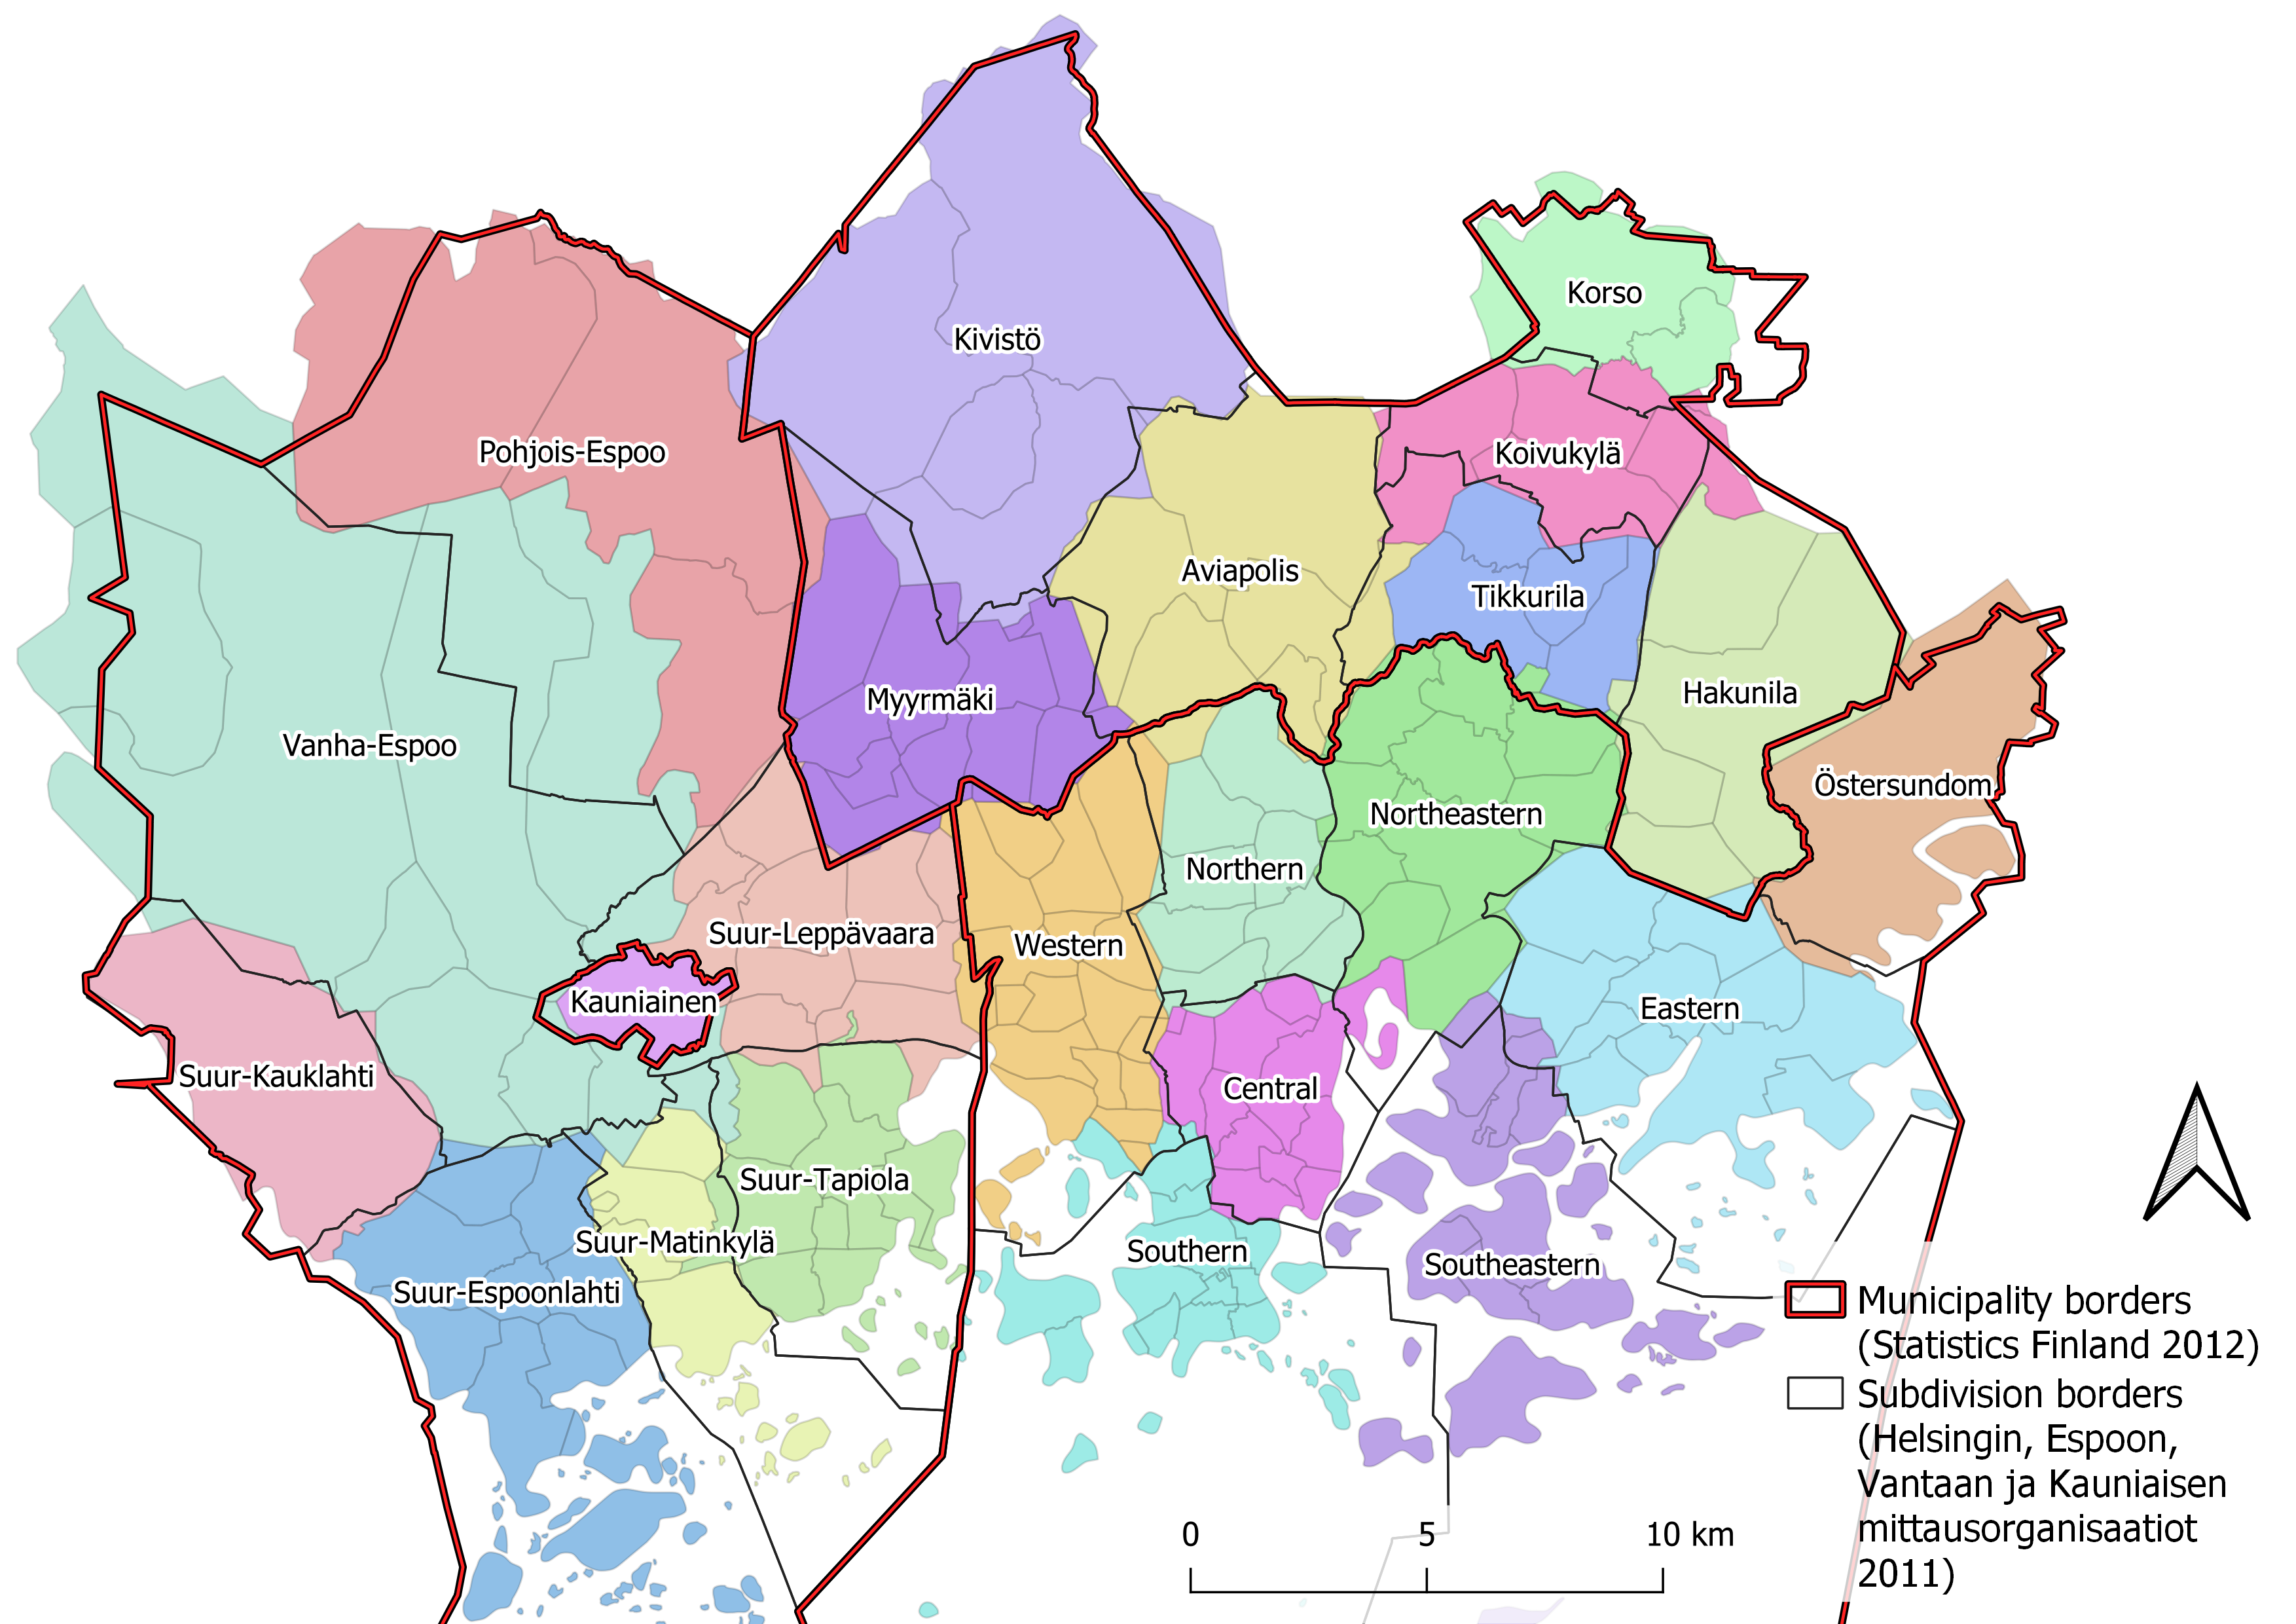
\includegraphics[width=\textwidth]{images/thesis_subdiv_place.png}
    \caption[Placing postal code areas in subdivisions]{For the purposes of analysis in R, all postal code areas in \textit{postal} were assigned with subdivision information. In this figure, distinct colors depict the postal code areas with the subdivision classification chosen for this thesis.}%
    \label{fig:subdiv_placement}%
\end{figure}

\newpage
\subsection{Creating applications and conducting analyses}
\subsubsection{Analysis application}
\justify
%\begin{itemize}
%    \item Prepare data to R compliant format
%    \item ShinyApp descriptive statistics
%    \item shinyapp histogram for parktime and walktime
%    \item shinyapp boxplot, show outliers
%    \item shinyapp barplot, show amounts
%    \item shinyapp levene test
%    \item shinyapp one-way anova
%    \item shinyapp map, nice to have, not at all important
%    \item visitor shinyapp, see the accumulation of visits and received records
%\end{itemize}

Once the data processing in Python was completed, \textit{records} and \textit{visitors} were carried over to R to utilise its easy to access statistical analysis functionality. For this thesis, this meant namely packages \textit{onewaytests} for ANOVA and Brown-Forsythe test, \textit{plotrix} for standard error, and \textit{moments} for quantiles (table~\ref{tab:used_soft}). To help study the large datasets, three Shiny applications were written, one for \textit{records} and a second for \textit{visitors}, and a third one to study differences between the thesis survey results and Helsinki Region Travel Time Matrix 2018. Benefits in creating these applications were twofold. Firstly, approaching the survey results from an interactive perspective allowed countless combinations of active and inactive variables -- without constant tweaking of code -- which would be beneficial for the analysis of \textit{records}. Secondly, programming the applications using Shiny enabled the use of shinyapps.io, a service where one can host Shiny applications on the internet without charge. Combination of these two factors made it effortless to analyse results of the survey in a visual way and at the same time, publish the tools and results to the public, upholding the thesis' mission of openness and transparency.

\begin{figure}[H]%
    \centering
    \subfloat[A segment of the shinyapps.io deployment of \textit{records} application. The web application provides a wide array of analysis and visualisation tools for the results of the thesis survey research.]{{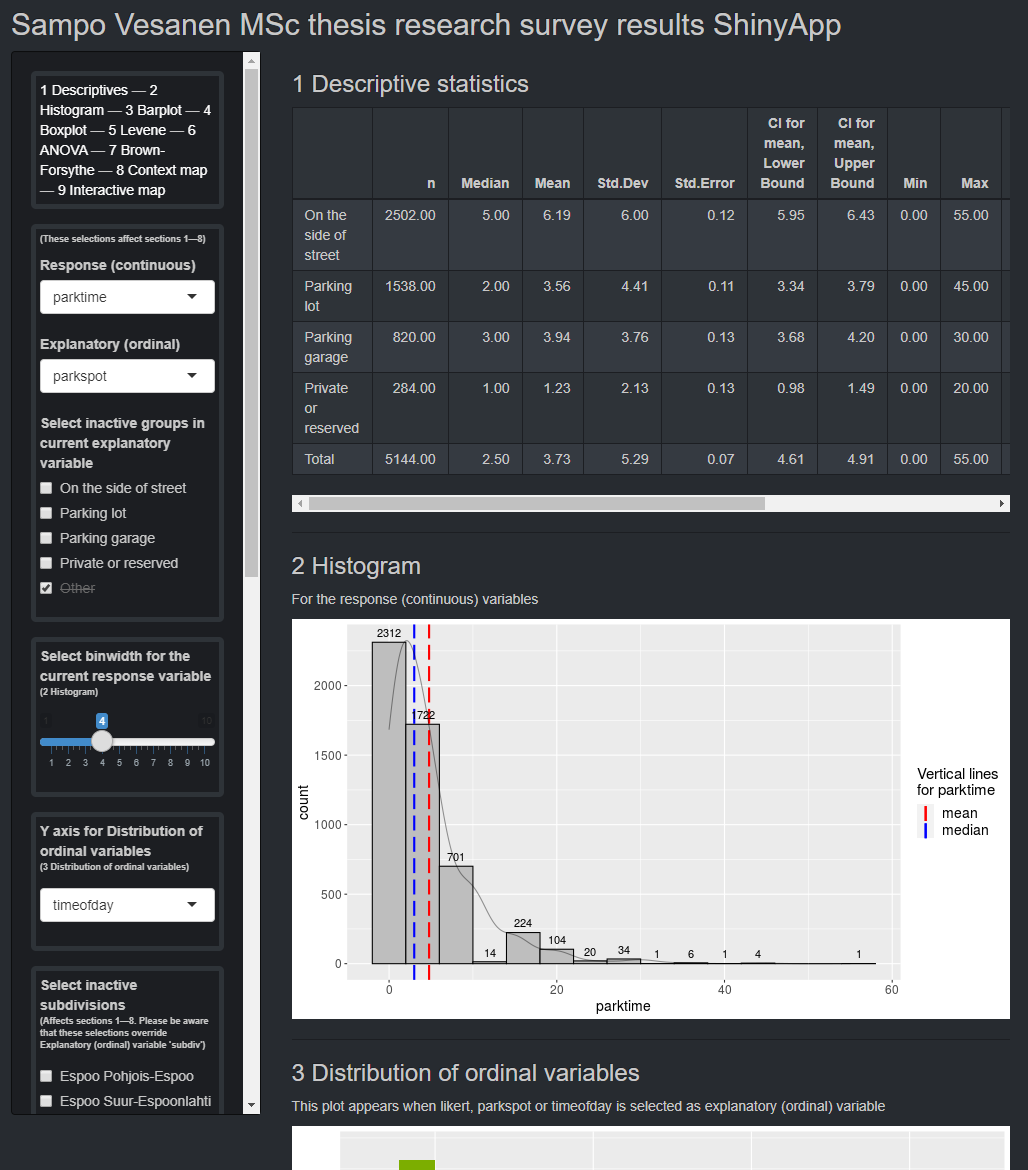
\includegraphics[width=8.1cm]{images/shinyapps_analysis.png} }}%
    \quad
    \subfloat[The shinyapps.io deployment of \textit{visitors} application. In this web application users may examine how the amounts of submitted responses and unique first visits to the thesis web survey developed over time.]{{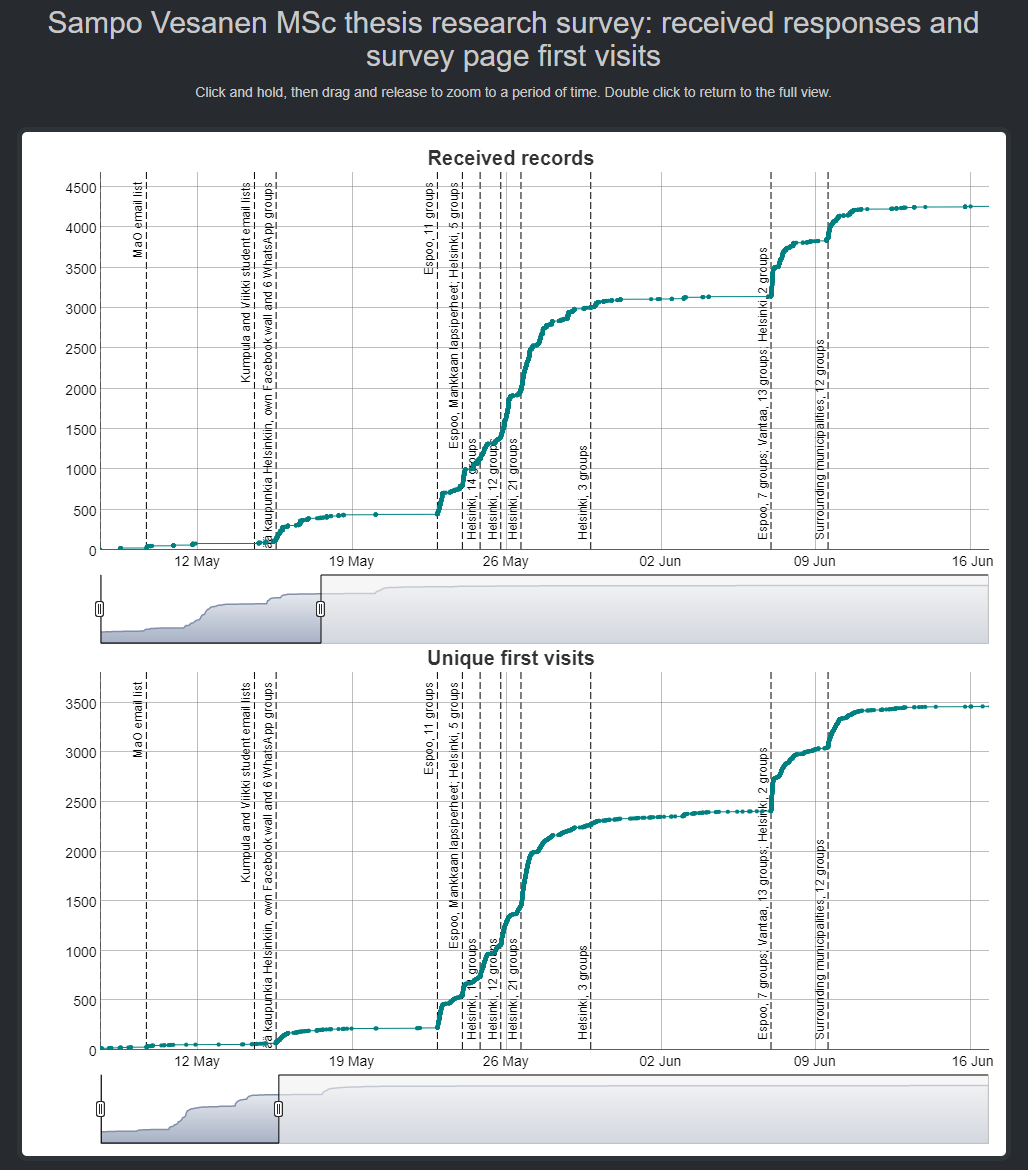
\includegraphics[width=8.1cm]{images/shinyapps_visitors.png} }}%
    \caption[Survey results as shinyapps.io web applications]{shinyapps.io deployments of the two survey dataset analysis applications.}%
    \label{fig:shinyapps}%
\end{figure}

In the Shiny application for \textit{records}, users can view the survey responses from many different angles. Users are given control which variables are active at any moment (\hyperref[fig:shinyapps]{figure~\ref{fig:shinyapps}a}). Users control the variables through the side panel, with settings taking effect in the main panel. The variables currently viewed are selected through two dropdown menus, Response (continuous) and Explanatory (ordinal). Continuous variables are \code{parktime} and \code{walktime} with an integer range 0--99. Available ordinal variables are \code{likert}, \code{parkspot}, \code{timeofday}, \code{artificial}, \code{ykr\_zone}, and \code{subdiv} with the values that can not be unequivocally ordered in a sequence in the same way as continuous variables. One variable from each variable group can be selected at the same time. Any and all groups of values in the ordinal variables can be deactivated to better understand the significance of each value group. In addition to the selection of the continuous and ordinal variable, users can deactivate \textit{records} data rows based on their spatial location in municipality subdivisions assigned in \hyperref[sec:processdata]{\fullref{sec:processdata}}. Most importantly, the analysis application allows selection of maximum allowed value for \code{parktime} and \code{walktime}. The default value for both is set at 59 minutes, as discussed in the \fullref{sec:processdata}, but the user is free to choose any value between zero and 99.

% levene, anova, boxplot, lue: https://www.itl.nist.gov/div898/handbook/eda/section3/eda35a.htm. On legit lähde
\begin{table}[H]
    \centering
    \caption[Records Shiny application features]{\textit{Records} Shiny application features. All features are affected by the maximum permitted \code{parktime} and \code{walktime} values, currently active response and explanatory variables and inactive subdivisions. In addition, certain exclusive settings are found in some of the features.}
    \label{tab:records_shiny_features}
    \scalebox{0.8}
    {\def\arraystretch{1.3}
    \setlength\tabcolsep{1.2ex}
    \begin{tabular}{ @{} >{\raggedright\arraybackslash}p{3cm} >{\raggedright\arraybackslash}p{2cm} >{\raggedright\arraybackslash}p{6cm} >{\raggedright\arraybackslash}p{6cm} @{} }
        \toprule
        Feature & Type & Outputs & Feature exclusive settings \\
        \midrule
        1 Descriptive statistics & Analysis, table & n, median, mean, standard deviation, standard error, confidence interval for mean, lower bound, confidence interval for mean, min, max, 25th quartile, 75th quartile, skewness, kurtosis & None \\
        2 Histogram & Analysis, chart & Histogram, kernel density estimate, mean, median & Histogram binwidth \\
        3 Distribution of ordinal variables & Analysis, chart & Distribution plot by explanatory variable value group & Explanatory variable for the distribution plot Y axis \\
        4 Boxplot & Analysis, chart & Quartile data & None \\
        5 Test of homogeneity of variances (Levene's test) & Analysis, table & Equality of variances for a variable calculated for the currently active response and explanatory variable & None \\
        6 Analysis of variance (ANOVA) & Analysis, table & Analysis of differences among group means in a sample & None \\
        7 Brown-Forsythe test & Analysis, table & Analysis of equality of group variances & None \\
        8 Interactive map & Visualisation, map & Choropleth map with Jenks breaks classifiction, descriptive data per postal code area (answer count, mean and median for parktime and walktime, forest amount percentage, largest YKR zone percentage) & - Selection of active municipalities \linebreak - Jenks breaks parameter column \linebreak - Amount of Jenks breaks classes \linebreak - Possibility to visualise the map with boundaries and labels \\
        \bottomrule
    \end{tabular}}
\end{table} 

When the user has selected a continuous and an ordinal variable to compare, they are presented a thorough set of descriptive statistics for the currently active data rows with n, median, mean, standard deviation, standard error, confidence interval for lower and upper bound, minimum and maximum, 25 \% and 75 \% quantiles, skewness, and kurtosis (table~\ref{tab:records_shiny_features}). For the continuous variables, a histogram is available to visualise the distribution of \code{walktime} and \code{parktime}. Distribution of ordinal variables \code{likert}, \code{parkspot}, and \code{timeofday} can be compared against other ordinal variables in a barplot. To study quartiles, a boxplot is available. Importantly, users can test their selection of variables with the test of homogeneity of variables (Levene's test), analysis of variance (ANOVA), and the Brown-Forsythe test \textcolor{red}{laajenna selityksiä}. Lastly, a versatile interactive map of the research area is provided. This map, divided in postal code areas, reveals the survey results in a spatial fashion. The interactive map is affected by the maximum parking time and walking time, selection of an ordinal variable and any inactive subdivisions to provide a flexible view into the details of the data. In addition, this interactive map is controlled by some exclusive settings of its own. The interactive map settings offers six distinct parameters for viewing the research area through Jenks natural breaks classification, alongside with the possibility to select the amount of classes in the map view. Hovering the cursor over the map reveals a tooltip which the application users can use to view mean, median, and percentage data about each postal code area in Helsinki Capital Region. Tooltips are also available for the barplot of distribution of ordinal variables and the boxplot.

Much additional work was put into the analysis application to make it as clear and easy to use as possible. The application features a number of links to move between the features and the settings, while smooth scrolling and animations help in directing the attention of the user. Each application feature can be switched on and off to make space for exactly the topic the user wants to examine. The analysis application allows downloading all the results, outputting tables into comma separated value files (CSV). Charts and the map are outputted into high resolution images (PNG). \textcolor{red}{too much detail?} \textcolor{purple}{The files are intuitively named informing of the used application settings and the date of file download. In case ordinal variable value groups or subdivisions are turned off, the output images are appended with an appropriate notification.} Attention was given to ensure the usage of the analysis application on mobile phones. To this end, the CSS style sheet of the application detects mobile phone screen sizes and adjusts the application content accordingly. The sidebar tends to block the view of the main panel on mobile screens and for this situation a switch is provided to hide the sidebar at any given time. All graphical elements of the application are in SVG (Scalable Vector Graphics) format which supports effortless zooming without loss of detail.

The source code for the \textit{records} analysis application is available at GitHub (\textcolor{blue}{\url{https://github.com/sampoves/thesis-records-shinyapps}}). The application may be viewed on shinyapps.io (\textcolor{blue}{\url{https://sampoves.shinyapps.io/records}}).

\subsubsection{Visitors application}

In the Shiny application for \textit{visitors}, users can examine events in the timeline of the survey research (figure~\ref{fig:shinyapps}). In this interactive view, cumulative charts are presented for received survey responses and survey page first visits. The charts reveal the effect and importance of advertisement on actual received responses and survey traffic. While not completely verifiable, the significance of different sources of responses can be viewed in the application.

Compared to the other two analysis applications programmed for this thesis, the \textit{visitors} application is relatively simple in its function and features. The user controls the chart view with mouse clicks or dragging the cursor and no additional settings are provided.

The source code for the \textit{visitors} analysis application is available at GitHub (\textcolor{blue}{\url{https://github.com/sampoves/thesis-visitors-shinyapps}}). The application may be viewed on shinyapps.io (\textcolor{blue}{\url{https://sampoves.shinyapps.io/visitors}}).

\subsubsection{Travel time comparison application}

Despite potential for extensive analysis, the applications described in previous chapters do not provide means to study the third research question of this thesis:

\begin{displayquote}
III What is the significance of the parking process to the overall travel time?
\end{displayquote}

To answer this research question, an application to compare travel time datasets was programmed (figure~\ref{fig:shinyapps_comparison}). In this application, the user can view a variety of descriptive values calculated from Helsinki Region Travel Time Matrix 2018, the thesis survey data, and a dataset created by comparing the two other datasets. The user is given control a set of features, such as the travel times origin postal area code, a parameter to visualise on the map, and the amount of symbology classes. The map view can be customised with a number of visualisation options, such as visible regional boundaries and physical features (inland water, main roads), and options for the labelling of postal code areas.

It was decided that the basic spatial unit for the comparison application would be the PAAVO postal code area as the thesis survey results exist in that resolution. This decision necessitated extensive processing of \textit{TTM} data. Firstly, the application needed to be able to recalculate the map view as quickly as possible. Secondly, the original \textit{TTM} dataset is unwieldy to be used in its original format in a web application (data stored in uncompressed txt files, data scope much too detailed for the application). Thirdly, the hosting service shinyapps.io places technical limitations on the resource intensity of the application. For these three main reasons, the library fst (table~\ref{tab:used_soft}) was first used to convert the \textit{TTM} private car columns into the data format used by the library (table~\ref{tab:comparison_fst1}), and then using the dataset \textit{grid} preprocessed in Python to aggregate all \textit{TTM} grid cell values to the PAAVO postal code area level and writing the results using the optimised fst format (table~\ref{tab:comparison_fst2}). For data completeness, \textit{TTM} searching for parking (0.42 minutes) and walking to destination (2.0--2.5 minutes) data was added to these aggregated \textit{TTM} files. This aggregation method drastically reduced unnecessary processing, minimised disk space needed, and kept application memory footprint in manageable figures for the deployment to the internet. The other main dataset used in the comparison application, the thesis survey data, is aggregated to postal code area level each time the application initialises, as the complete survey results dataset is miniscule in size compared to \textit{TTM}.

\begin{hyphenrules}{nohyphenation}
    \begin{table}[H]
        \centering
        \setlength\tabcolsep{1pt}
        \caption[Comparison application fst structure I]{An excerpt of the data content of \textit{TTM} converted to fst format for further processing (table~\ref{tab:comparison_fst2}). Original file 5785xxx/travel\_times\_to\_ 5785640.txt.} 
        \label{tab:comparison_fst1}
        \begin{tabular}{ @{} >{\raggedright\arraybackslash}p{1cm} >{\raggedright\arraybackslash}p{2cm} >{\raggedright\arraybackslash}p{2cm} >{\raggedright\arraybackslash}p{2cm} >{\raggedright\arraybackslash}p{2cm} >{\raggedright\arraybackslash}p{2cm} @{} }
            \toprule
            & from\_id & to\_id & car\_r\_t & car\_m\_t & car\_sl\_t \\
            \midrule
            10 & 5787549 & 5785640 & 22 & 21 & 16 \\
            11 & 5787550 & 5785640 & 22 & 21 & 16 \\
            12 & 5789447 & 5785640 & 10 & 9 & 8 \\
            13 & 5789448 & 5785640 & 10 & 9 & 8 \\
            14 & 5789449 & 5785640 & 11 & 10 & 9 \\
            \bottomrule
        \end{tabular}
    \end{table} 
\end{hyphenrules}

\begin{hyphenrules}{nohyphenation}
    \begin{table}[H]
        \centering
        \setlength\tabcolsep{5pt}
        \caption[Comparison application fst structure II]{An excerpt of the data content of \textit{TTM} aggregated to postal code area level for the use of the comparison application. The origin postal code area of the shown data table is 00100 Helsinki Keskusta -- Etu-Töölö.} 
        \label{tab:comparison_fst2}
        \begin{tabular}{ @{} >{\raggedright\arraybackslash}p{1cm} >{\raggedright\arraybackslash}p{1.5cm} >{\raggedright\arraybackslash}p{1.5cm} >{\raggedright\arraybackslash}p{2cm} >{\raggedright\arraybackslash}p{2cm} >{\raggedright\arraybackslash}p{2cm} >{\raggedright\arraybackslash}p{2cm} >{\raggedright\arraybackslash}p{2cm} @{} }
            \toprule
            & zipcode & from\_zip & ttm\_r\_avg & ttm\_m\_avg & ttm\_sl\_avg & ttm\_wtd & ttm\_sfp \\
            \midrule
            5 & 00150 & 00100 & 14.89 & 13.24 & 9.48 & 2.33 & 0.42 \\
            6 & 00160 & 00100 & 15.48 & 13.97 & 9.77 & 2.50 & 0.42 \\
            7 & 00170 & 00100 & 14.41 & 13.10 & 9.09 & 2.50 & 0.42 \\
            8 & 00180 & 00100 & 12.77 & 11.34 & 8.40 & 2.50 & 0.42 \\
            9 & 00190 & 00100 & 24.27 & 22.31 & 17.04 & 2.00 & 0.42 \\
            \bottomrule
        \end{tabular}
    \end{table} 
\end{hyphenrules}

\begin{hyphenrules}{nohyphenation}
    \begin{table}[H]
        \centering
        \def\arraystretch{1.2}
        \setlength\tabcolsep{5pt}
        \caption[Comparison application tooltip content]{Comparison application tooltip content meaning. All values are per postal code area.} 
        \label{tab:comparison_tooltip_content}
        \scalebox{0.8}
        {\begin{tabular}{ @{} >{\raggedright\arraybackslash}p{2cm} >{\raggedright\arraybackslash}p{2cm} >{\raggedright\arraybackslash}p{9.0cm} >{\raggedright\arraybackslash}p{5.5cm} @{} }
            \toprule
            & Column name, unit & Description & Formula \\
            \midrule
            \multirow{3}{3cm}[-1ex]{timeofday} & r & Rush hour traffic (09:00–11.00, 15.00–17.00) & -- \\
            & m & Midday traffic (09.00–15.00) & -- \\
            & all & An average of all available data. For \textit{TTM}, these are Rush hour traffic, Midday traffic, and Route following speed limits without any additional impedances. For thesis survey data, these are the values of the survey question timeofday: Weekday, rush hour, Weekday, other than rush hour, Weekend, and Can't specify, no usual time. & $\frac{value_1 + value_2 + ... + value_n}{n}$ \\
            \greyrule
            
            \multirow{5}{3cm}[-1ex]{Travel Time Matrix 2018} & sfp, min & Time consumed in searching for parking. In \textit{TTM}, this is 0.42 minutes for all YKR IDs in the entirety of Helsinki Capital Region (\cite{Toivonen2014a}). & -- \\
            & wtd\_avg, min & An averaged value of walking time from one's parked private car to the final destination of the travel chain. In \textit{TTM}, this is 2.0 minutes for all \textit{grid} cells in the entirety of Helsinki Capital Region, except in a square defined over the center of Helsinki, where the value is 2.5 minutes for all \textit{grid} cells (\cite{Toivonen2014a}). & -- \\
            & avg, min & A mean duration of the complete travel chain with private car from origin postal code area to the destination postal code area. & $\frac{car\_x\_t_1 + car\_x\_t_2 + ... + car\_x\_t_n}{n}$, where $x$ is $r$, $m$, or $all$. $car\_$ represents unchanged \textit{TTM} data columns. \\
            & drivetime, min & The length of the driving segment of the mean duration of the complete travel chain from origin postal code area to the destination postal code area without searching for parking (using the \textit{TTM} value) or walking to the final destination of the travel chain (\textit{TTM} value). & $ttm\_x\_avg - ttm\_sfp - ttm\_wtd\_avg$ \\
            & pct, \% & How much does searching for parking and walking from one's parked car to the final destination of the travel chain constitute of the mean duration of the complete travel chain? & $\frac{ttm\_sfp + ttm\_wtd\_avg}{ttm\_x\_avg}$ \\
            \greyrule
            
            \multirow{4}{3cm}[-1ex]{Thesis data} & sfp\_avg, min & Time consumed, on average, in searching for parking in a postal code area, according to the thesis survey respondents. & $\frac{parktime_1 + parktime_2 + ... + parktime_n}{n}$, while postal code value is constant. \\
            & wtd\_avg, min & Average walking time from one's parked private car to the final destination in a postal code area, according to the thesis survey respondents. & $\frac{walktime_1 + walktime_2 + ... + walktime_n}{n}$, while postal code value is constant. \\
            & drivetime, min & The length of the driving segment of the mean duration of the complete travel chain (\textit{TTM} data) from the origin postal code area to the destination postal code area, without searching for parking (thesis survey mean) or walking to destination (thesis survey mean). & $ttm\_x\_avg - thesis\_x\_sfp - thesis\_x\_wtd$, where $x$ is $r$, $m$, or $all$. \\
            & pct, \% & How much do the thesis mean values for searching for parking and walking from one's parked car to the final destination constitute of the mean duration of the complete travel chain? & $\frac{(thesis\_x\_sfp + thesis\_x\_wtd)}{ttm\_x\_avg}$ \\
            \greyrule
            
            \multirow{4}{3cm}[-1ex]{Compare TTM and thesis} & sfp, \% & Compare \textit{TTM} and thesis survey values for searching for parking. & $\frac{thesis\_x\_sfp}{ttm\_sfp}$, where $x$ is $r$, $m$, or $all$. \\
            & wtd, \% & Compare \textit{TTM} and thesis survey values for the duration to walk from one's parked car to the final destination of the travel chain. & $\frac{thesis\_x\_wtd}{ttm\_wtd\_avg}$ \\
            & drivetime, \% & Compare the driving time segment of the mean duration of the complete travel chain in TTM and thesis data. & $\frac{thesis\_x\_drivetime}{ttm\_x\_drivetime}$ \\
            & pct, \% & Compare the percentual value of the significance of searching for parking and walking to one's final destination of the mean duration of the complete travel chain in \textit{TTM} and thesis data. & $\frac{thesis\_x\_pct}{ttm\_x\_pct}$ \\
            \bottomrule
        \end{tabular}}
    \end{table} 
\end{hyphenrules}

\begin{figure}[H]%
    \centering
    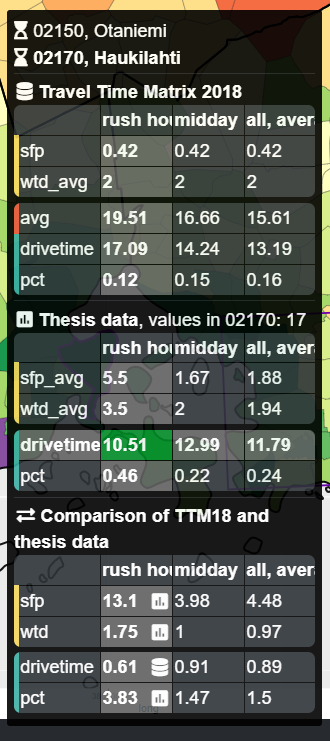
\includegraphics[width=0.33\textwidth]{images/shinyapps_comparison_detail.png}
    \caption[Comparison application data]{Close-up of a tooltip for a travel chain from 02150 Otaniemi to 02170 Haukilahti. The cell coloured green tells the user that currently visualised on map is thesis data, the travel chain without searching for parking or walking to one's destination, in rush hour traffic.}%
    \label{fig:shinyapps_comparison_detail}%
\end{figure}

\begin{figure}[H]%
    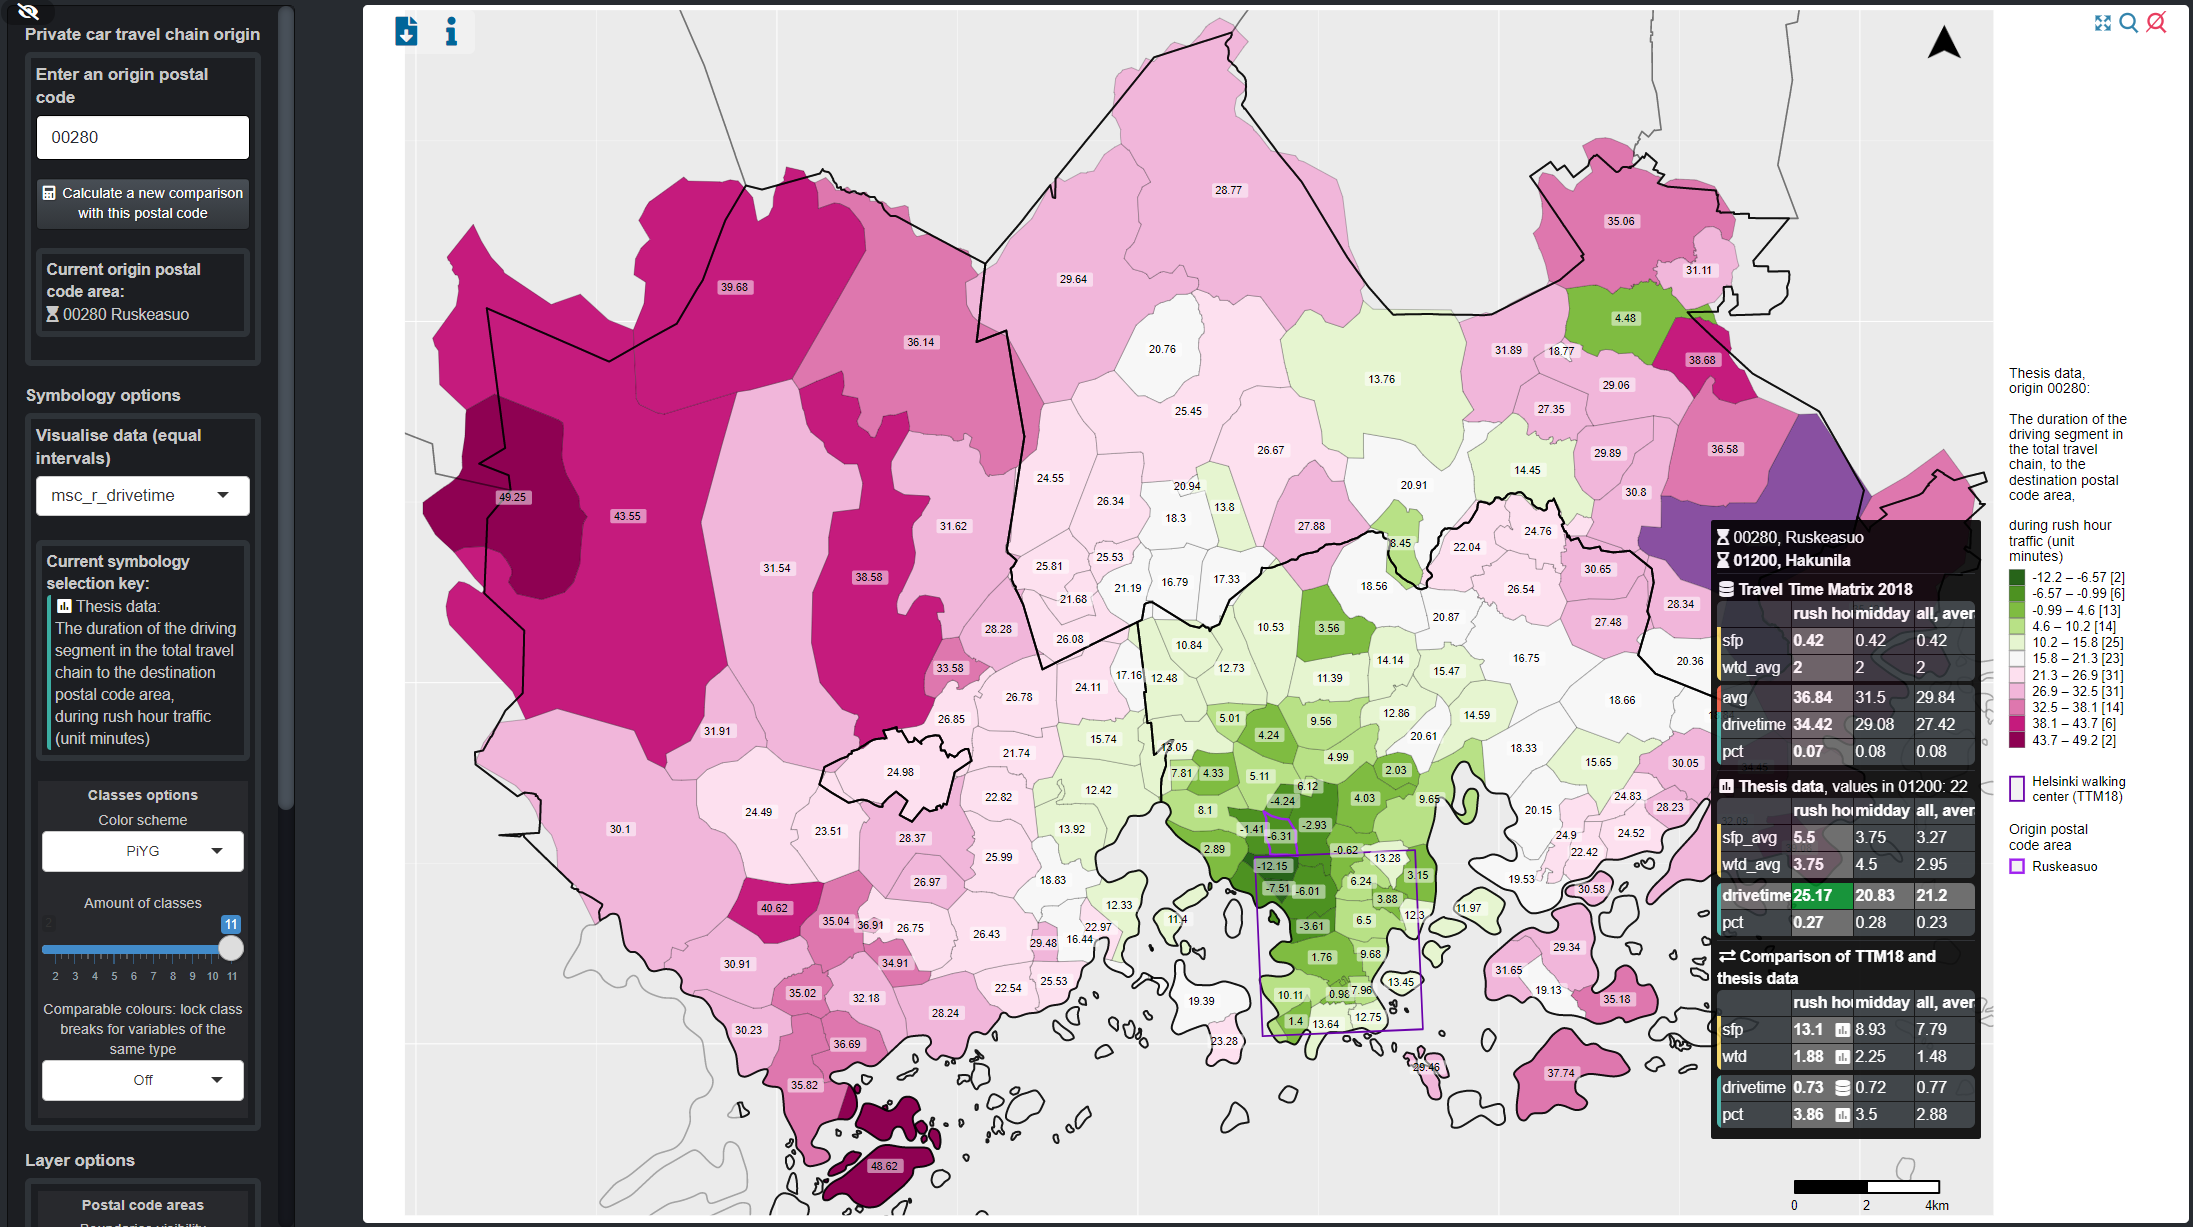
\includegraphics[width=\textwidth]{images/shinyapps_comparison.png}
    \caption[Comparison application screenshot]{Helsinki Region Travel Time Matrix 2018 and thesis survey data comparison application's shinyapps.io deployment. The cursor hovers over 01200 Hakunila with the appropriate tooltip shown.}%
    \label{fig:shinyapps_comparison}%
\end{figure}

The source code for the travel time comparison application is available at GitHub (\textcolor{blue}{\url{https://github.com/sampoves/thesis-comparison-shinyapps}}). The application may be viewed on shinyapps.io (\textcolor{blue}{\url{https://sampoves.shinyapps.io/comparison}}).